\documentclass{article} % use larger type; default would be 10pt

\usepackage{pgfplots}
\usetikzlibrary{calc}
\usetikzlibrary{arrows}
\usetikzlibrary{patterns}
\usetikzlibrary{calc,intersections,through,backgrounds}
\usetikzlibrary{decorations.pathreplacing}
        \newcommand\degree[0]{^{\circ}}
        \newcommand\abs[1]{\left|#1\right|}

\title{Play with TikZ}
\author{Just Us}
%\date{} % Activate to display a given date or no date (if empty),
         % otherwise the current date is printed 

\begin{document}
\maketitle

\section{Chap 3 Section 1}



fig-3-1-1


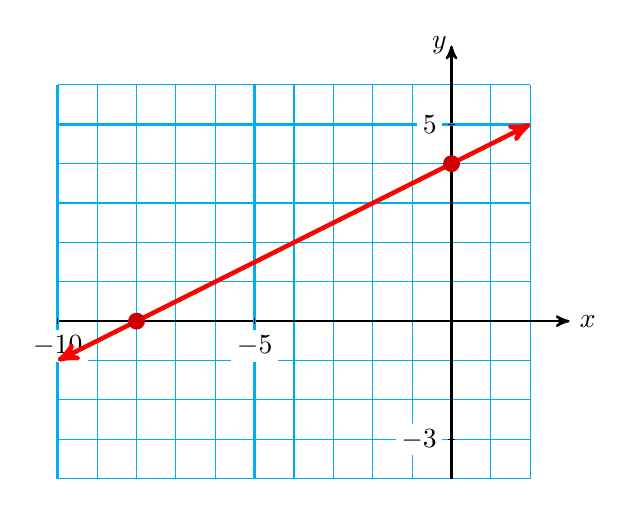
\begin{tikzpicture} [scale=0.5]
\draw[cyan] (-10,-4) grid (2,6);
\draw[black,thick, ->, >=stealth'] (-10,0)--(3,0) node[right]{$x$};
\draw[black,thick, ->, >=stealth'] (0,-4)--(0,7) node[left, xshift=2]{$y$};
\foreach \x in  {-10,-5} {
 \draw[cyan,very thick] (\x,-4) --(\x,6); 
 \draw[black] (\x,.08) --++(0,-.16)  node[below, yshift=-2, fill=white, inner sep=2]   {$\x$};
}
\draw[cyan, very thick] (-10,5) --(2,5); 
\foreach \y  in  {-3,5} {
 \draw[black] (.08,\y) --++(-.16,0)  node[left, xshift=-2, fill=white, inner sep=2] {$\y$};
}
\draw[red, ultra thick, <->, >=stealth'] (-10,-1)--(2,5);
\filldraw[red!80!black] (-8,0) circle (2mm);
\filldraw[red!80!black] (0,4) circle (2mm);
\end{tikzpicture}
\newline

fig-3-1-ex2 line and intercepts


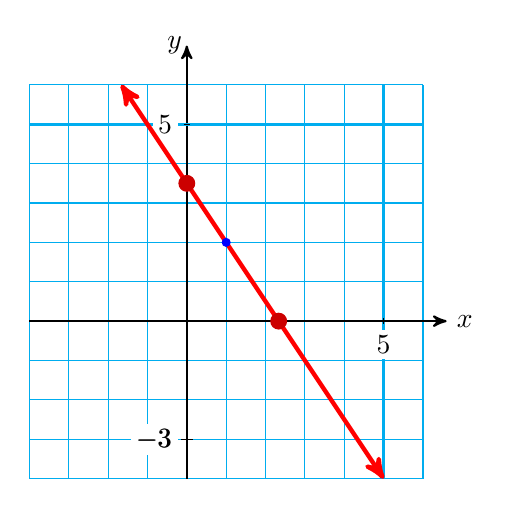
\begin{tikzpicture} [scale=0.5]
\draw[cyan] (-4,-4) grid (6,6);
 \draw[cyan,very thick] (5,-4) --(5,6); 
\draw[black,thick, ->, >=stealth'] (-4,0)--(6.6,0) node[right]{$x$};
\draw[black,thick, ->, >=stealth'] (0,-4)--(0,7) node[left, xshift=2]{$y$};
\foreach \x in  {5} {
 \draw[black] (\x,.08) --++(0,-.16)  node[below, yshift=-2, fill=white, inner sep=2]   {$\x$};
}
\draw[cyan, very thick] (-4,5) --(6,5); 
\foreach \y  in  {-3,5} {
 \draw[black] (.08,\y) --++(-.16,0)  node[left, xshift=-2, fill=white, inner sep=2]   {$\y$};
}
 \draw[black] (.15,-3) --++(-.3,0)  node[left]   {$-3$};
\draw[red, ultra thick, <->, >=stealth'] (-5/3,6)--(5,-4);
\filldraw[red!80!black] (7/3,0) circle (2mm);
\filldraw[red!80!black] (0,7/2) circle (2mm);
\filldraw[blue] (1,2) circle (1mm);
\end{tikzpicture}
\newline


fig-3-1-ex3 line and intercepts

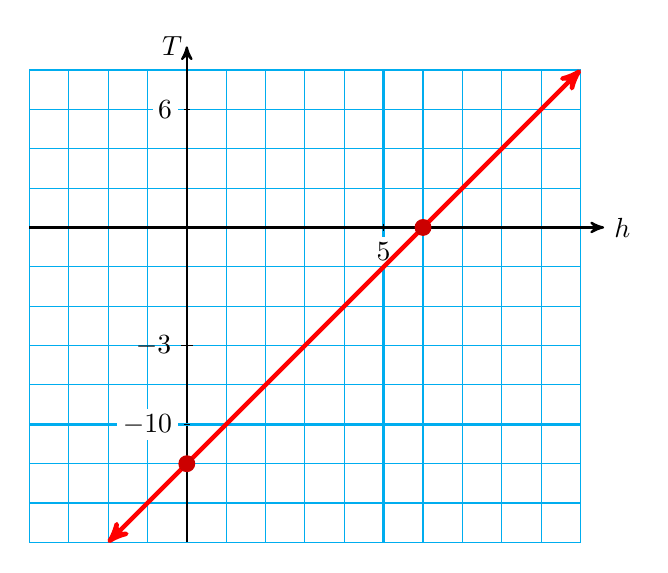
\begin{tikzpicture} [scale=0.5]
\draw[cyan] (-4,-8) grid (10,4);
\draw[cyan,very thick] (5,-8) --(5,4); 
\draw[black,thick, ->, >=stealth'] (-4,0)--(10.6,0) node[right]{$h$};
\draw[black,thick, ->, >=stealth'] (0,-8)--(0,4.6) node[left, xshift=2]{$T$};
\foreach \x in  {5} {
 \draw[black] (\x,.08) --++(0,-.16)  node[below, yshift=-2, fill=white, inner sep=2]   {$\x$};
}
\draw[cyan, very thick] (-4,-5) --(10,-5); 
\foreach \y [evaluate=\y as \yi using int(2*\y)] in  {-5,3} {
 \draw[black] (.08,\y) --++(-.16,0)  node[left, xshift=-2, fill=white, inner sep=2]   {$\yi$};
}
 \draw[black] (.15,-3) --++(-.3,0)  node[left]   {$-3$};
\draw[red, ultra thick, <->, >=stealth'] (-2,-8)--(10,4);
\filldraw[red!80!black] (6,0) circle (2mm);
\filldraw[red!80!black] (0,-6) circle (2mm);
\end{tikzpicture}
\newline


10 by 10 grid: hp-2-3-12


hp-3-1-1ans

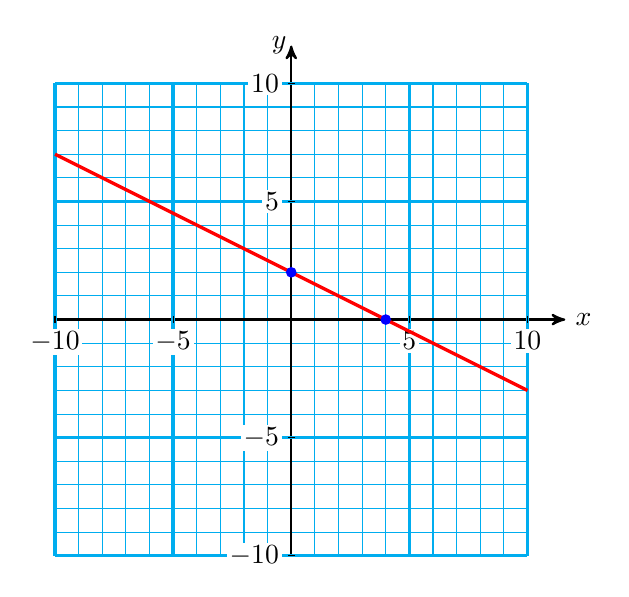
\begin{tikzpicture} [scale=.3]
\coordinate (O) at (0,0);
\draw[cyan] (-10,-10) grid (10,10);
\draw[black,thick, ->, >=stealth'] (-10,0)--(11.6,0) node[right]{$x$};
\draw[black,thick, ->, >=stealth'] (0,-10)--(0,11.6) node[left, xshift=2]{$y$};
\foreach \x in  {-5, 5, -10, 10} {
 \draw[cyan, very thick] (\x,-10) --++(0,20);
 \draw[cyan, very thick] (-10,\x) --++(20,0);
 \draw[black] (\x,.15) --++(0,-.3)  node[below, yshift=-2, fill=white, inner sep=1]   {$\x$};
 \draw[black] (.15,\x) --++(-.3,0)  node[left, xshift=-2, fill=white, inner sep=1]   {$\x$};
}
\draw[red,very thick] (-10,7)--(10,-3);
\filldraw[blue] (0,2) circle (2mm);
\filldraw[blue] (4,0) circle (2mm);
\end{tikzpicture}
\newline


hp-3-1-3ans

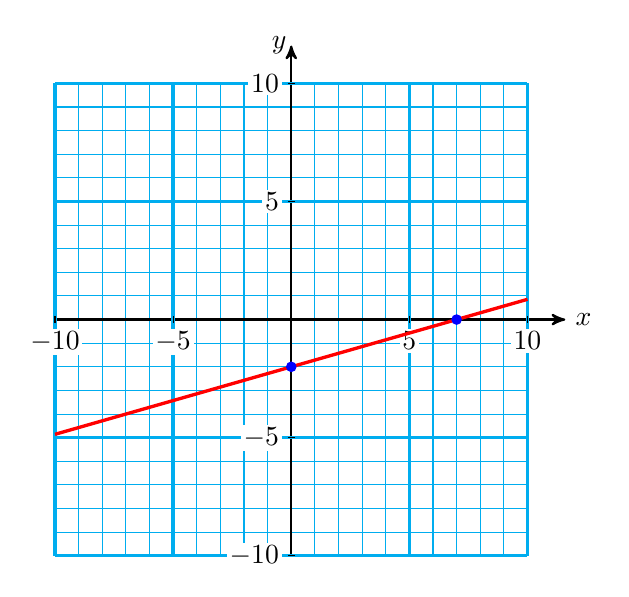
\begin{tikzpicture} [scale=.3]
\coordinate (O) at (0,0);
\draw[cyan] (-10,-10) grid (10,10);
\draw[black,thick, ->, >=stealth'] (-10,0)--(11.6,0) node[right]{$x$};
\draw[black,thick, ->, >=stealth'] (0,-10)--(0,11.6) node[left, xshift=2]{$y$};
\foreach \x in  {-5, 5, -10, 10} {
 \draw[cyan, very thick] (\x,-10) --++(0,20);
 \draw[cyan, very thick] (-10,\x) --++(20,0);
 \draw[black] (\x,.15) --++(0,-.3)  node[below, yshift=-2, fill=white, inner sep=1]   {$\x$};
 \draw[black] (.15,\x) --++(-.3,0)  node[left, xshift=-2, fill=white, inner sep=1]   {$\x$};
}
\draw[red,very thick] (-10,-34/7)--(10,6/7);
\filldraw[blue] (0,-2) circle (2mm);
\filldraw[blue] (7,0) circle (2mm);
\end{tikzpicture}
\newline



hp-3-1-5 50-by-50 grid

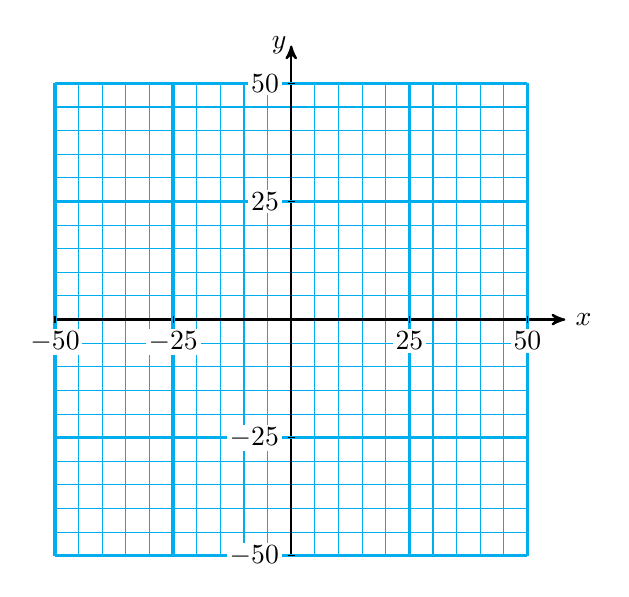
\begin{tikzpicture} [scale=.3]
\coordinate (O) at (0,0);
\draw[cyan] (-10,-10) grid (10,10);
\draw[black,thick, ->, >=stealth'] (-10,0)--(11.6,0) node[right]{$x$};
\draw[black,thick, ->, >=stealth'] (0,-10)--(0,11.6) node[left, xshift=2]{$y$};
\foreach \x [evaluate=\x as \xi using int(5*\x)] in  {-5, 5, -10, 10} {
 \draw[cyan, very thick] (\x,-10) --++(0,20);
 \draw[cyan, very thick] (-10,\x) --++(20,0);
 \draw[black] (\x,.15) --++(0,-.3)  node[below, yshift=-2, fill=white, inner sep=1]   {$\xi$};
 \draw[black] (.15,\x) --++(-.3,0)  node[left, xshift=-2, fill=white, inner sep=1]   {$\xi$};
}
\end{tikzpicture}
\newline



hp-3-1-5ans

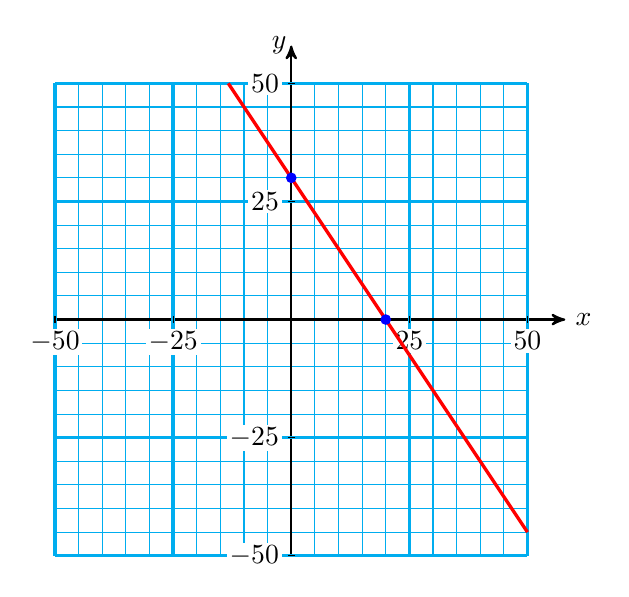
\begin{tikzpicture} [scale=.3]
\coordinate (O) at (0,0);
\draw[cyan] (-10,-10) grid (10,10);
\draw[black,thick, ->, >=stealth'] (-10,0)--(11.6,0) node[right]{$x$};
\draw[black,thick, ->, >=stealth'] (0,-10)--(0,11.6) node[left, xshift=2]{$y$};
\foreach \x [evaluate=\x as \xi using int(5*\x)] in  {-5, 5, -10, 10} {
 \draw[cyan, very thick] (\x,-10) --++(0,20);
 \draw[cyan, very thick] (-10,\x) --++(20,0);
 \draw[black] (\x,.15) --++(0,-.3)  node[below, yshift=-2, fill=white, inner sep=1]   {$\xi$};
 \draw[black] (.15,\x) --++(-.3,0)  node[left, xshift=-2, fill=white, inner sep=1]   {$\xi$};
}
\draw[red,very thick] (-8/3,10)--(10,-9);
\filldraw[blue] (0,6) circle (2mm);
\filldraw[blue] (4,0) circle (2mm);
\end{tikzpicture}
\newline


hp-3-1-6 100-by-100 grid

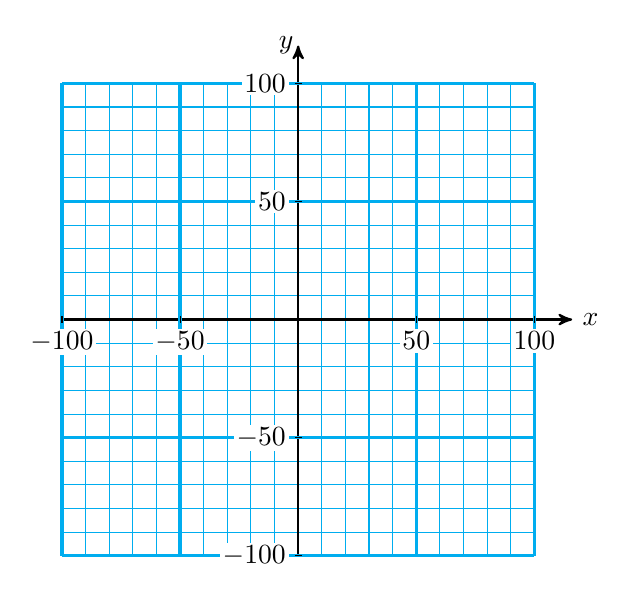
\begin{tikzpicture} [scale=.3]
\coordinate (O) at (0,0);
\draw[cyan] (-10,-10) grid (10,10);
\draw[black,thick, ->, >=stealth'] (-10,0)--(11.6,0) node[right]{$x$};
\draw[black,thick, ->, >=stealth'] (0,-10)--(0,11.6) node[left, xshift=2]{$y$};
\foreach \x [evaluate=\x as \xi using int(10*\x)] in  {-5, 5, -10, 10} {
 \draw[cyan, very thick] (\x,-10) --++(0,20);
 \draw[cyan, very thick] (-10,\x) --++(20,0);
 \draw[black] (\x,.15) --++(0,-.3)  node[below, yshift=-2, fill=white, inner sep=1]   {$\xi$};
 \draw[black] (.15,\x) --++(-.3,0)  node[left, xshift=-2, fill=white, inner sep=1]   {$\xi$};
}
\end{tikzpicture}
\newline


hp-3-1-7a 8 by 8 grid

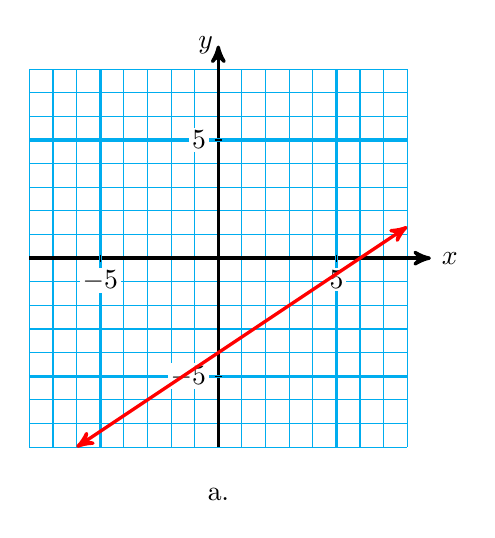
\begin{tikzpicture} [scale=.3]
\coordinate (O) at (0,0);
\draw[cyan] (-8,-8) grid (8,8);
\draw[black,very thick, ->, >=stealth'] (-8,0)--(9,0) node[right]{$x$};
\draw[black,very thick, ->, >=stealth'] (0,-8)--(0,9) node[left, xshift=2]{$y$};
\foreach \x  in  {-5, 5} {
 \draw[cyan, very thick] (\x,-8) --++(0,16);
 \draw[cyan, very thick] (-8,\x) --++(16,0);
 \draw[black] (\x,.15) --++(0,-.3) node[below, yshift=-2, fill=white, inner sep=1]   {$\x$};
 \draw[black] (.15,\x) --++(-.3,0) node[left, xshift=-2, fill=white, inner sep=1]   {$\x$};
}
\draw[red,very thick, <->, >=stealth'] (-6,-8)--(8,4/3);
\node at (0,-10) {a.};
\end{tikzpicture}
\newline


hp-3-1-7b 8 by 8 grid

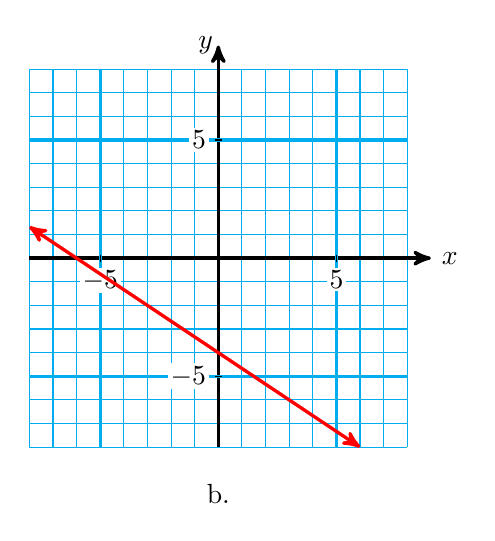
\begin{tikzpicture} [scale=.3]
\coordinate (O) at (0,0);
\draw[cyan] (-8,-8) grid (8,8);
\draw[black,very thick, ->, >=stealth'] (-8,0)--(9,0) node[right]{$x$};
\draw[black,very thick, ->, >=stealth'] (0,-8)--(0,9) node[left, xshift=2]{$y$};
\foreach \x  in  {-5, 5} {
 \draw[cyan, very thick] (\x,-8) --++(0,16);
 \draw[cyan, very thick] (-8,\x) --++(16,0);
 \draw[black] (\x,.15) --++(0,-.3) node[below, yshift=-2, fill=white, inner sep=1]   {$\x$};
 \draw[black] (.15,\x) --++(-.3,0) node[left, xshift=-2, fill=white, inner sep=1]   {$\x$};
}
\draw[red,very thick, <->, >=stealth'] (-8,4/3)--(6,-8);
\node at (0,-10) {b.};
\end{tikzpicture}
\newline


hp-3-1-7c 8 by 8 grid

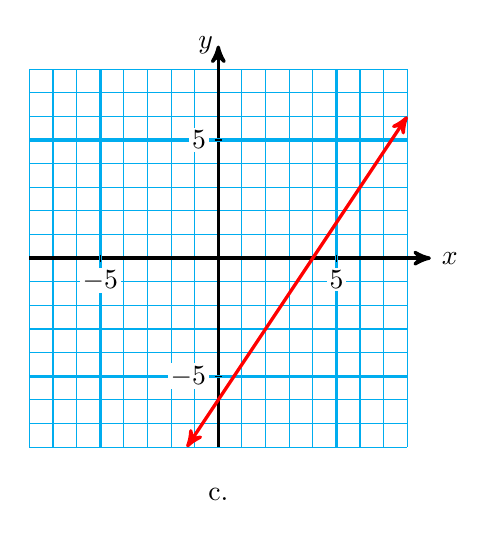
\begin{tikzpicture} [scale=.3]
\coordinate (O) at (0,0);
\draw[cyan] (-8,-8) grid (8,8);
\draw[black,very thick, ->, >=stealth'] (-8,0)--(9,0) node[right]{$x$};
\draw[black,very thick, ->, >=stealth'] (0,-8)--(0,9) node[left, xshift=2]{$y$};
\foreach \x  in  {-5, 5} {
 \draw[cyan, very thick] (\x,-8) --++(0,16);
 \draw[cyan, very thick] (-8,\x) --++(16,0);
 \draw[black] (\x,.15) --++(0,-.3) node[below, yshift=-2, fill=white, inner sep=1]   {$\x$};
 \draw[black] (.15,\x) --++(-.3,0) node[left, xshift=-2, fill=white, inner sep=1]   {$\x$};
}
\draw[red,very thick, <->, >=stealth'] (-4/3,-8)--(8,6);
\node at (0,-10) {c.};
\end{tikzpicture}
\newline


hp-3-1-7d 8 by 8 grid

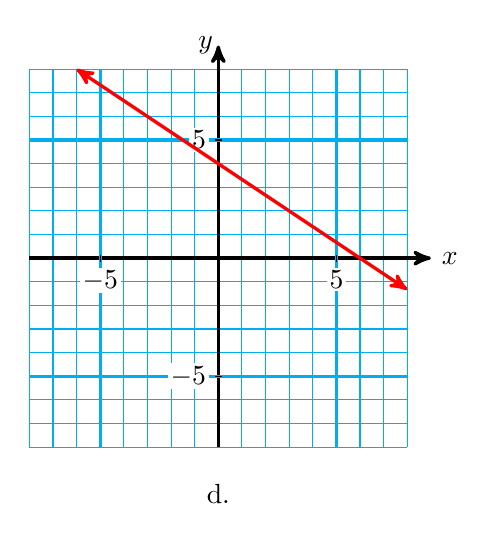
\begin{tikzpicture} [scale=.3]
\coordinate (O) at (0,0);
\draw[cyan] (-8,-8) grid (8,8);
\draw[black,very thick, ->, >=stealth'] (-8,0)--(9,0) node[right]{$x$};
\draw[black,very thick, ->, >=stealth'] (0,-8)--(0,9) node[left, xshift=2]{$y$};
\foreach \x  in  {-5, 5} {
 \draw[cyan, very thick] (\x,-8) --++(0,16);
 \draw[cyan, very thick] (-8,\x) --++(16,0);
 \draw[black] (\x,.15) --++(0,-.3) node[below, yshift=-2, fill=white, inner sep=1]   {$\x$};
 \draw[black] (.15,\x) --++(-.3,0) node[left, xshift=-2, fill=white, inner sep=1]   {$\x$};
}
\draw[red,very thick, <->, >=stealth'] (-6,8)--(8,-4/3);
\node at (0,-10) {d.};
\end{tikzpicture}
\newline


hp-3-1-7e 8 by 8 grid

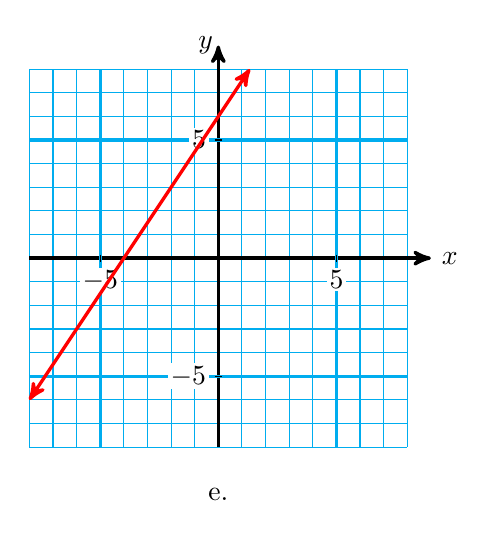
\begin{tikzpicture} [scale=.3]
\coordinate (O) at (0,0);
\draw[cyan] (-8,-8) grid (8,8);
\draw[black,very thick, ->, >=stealth'] (-8,0)--(9,0) node[right]{$x$};
\draw[black,very thick, ->, >=stealth'] (0,-8)--(0,9) node[left, xshift=2]{$y$};
\foreach \x  in  {-5, 5} {
 \draw[cyan, very thick] (\x,-8) --++(0,16);
 \draw[cyan, very thick] (-8,\x) --++(16,0);
 \draw[black] (\x,.15) --++(0,-.3) node[below, yshift=-2, fill=white, inner sep=1]   {$\x$};
 \draw[black] (.15,\x) --++(-.3,0) node[left, xshift=-2, fill=white, inner sep=1]   {$\x$};
}
\draw[red,very thick, <->, >=stealth'] (-8,-6)--(4/3,8);
\node at (0,-10) {e.};
\end{tikzpicture}
\newline


hp-3-1-7f 8 by 8 grid

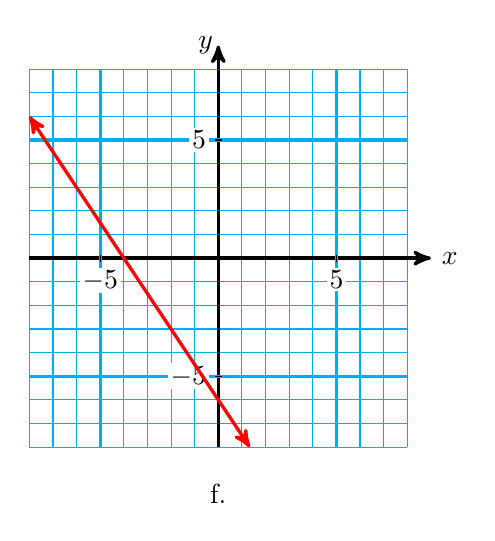
\begin{tikzpicture} [scale=.3]
\coordinate (O) at (0,0);
\draw[cyan] (-8,-8) grid (8,8);
\draw[black,very thick, ->, >=stealth'] (-8,0)--(9,0) node[right]{$x$};
\draw[black,very thick, ->, >=stealth'] (0,-8)--(0,9) node[left, xshift=2]{$y$};
\foreach \x  in  {-5, 5} {
 \draw[cyan, very thick] (\x,-8) --++(0,16);
 \draw[cyan, very thick] (-8,\x) --++(16,0);
 \draw[black] (\x,.15) --++(0,-.3) node[below, yshift=-2, fill=white, inner sep=1]   {$\x$};
 \draw[black] (.15,\x) --++(-.3,0) node[left, xshift=-2, fill=white, inner sep=1]   {$\x$};
}
\draw[red,very thick, <->, >=stealth'] (-8,6)--(4/3,-8);
\node at (0,-10) {f.};
\end{tikzpicture}
\newline


hp-3-1-19 grid

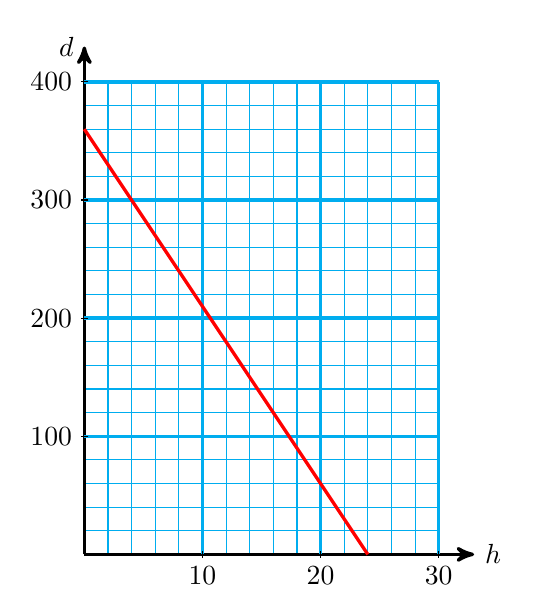
\begin{tikzpicture} [scale=.3]
\coordinate (O) at (0,0);
\draw[cyan] (O) grid (15,20);
\draw[black,very thick, ->, >=stealth'] (O)--(16.5,0) node[right]{$h$};
\draw[black,very thick, ->, >=stealth'] (O)--(0,21.5) node[left]{$d$};
\foreach \x [evaluate=\x as \xi using int(2*\x] in  {5,10,15} {
 \draw[cyan, very thick] (\x,0) --++(0,20);
 \draw[black] (\x,.15) --++(0,-.3) node[below, yshift=-2, fill=white, inner sep=1]   {$\xi$};
}
\foreach \x [evaluate=\x as \xi using int(20*\x] in  {5,10,15,20} {
 \draw[cyan, very thick] (0,\x) --++(15,0);
 \draw[black] (.15,\x) --++(-.3,0) node[left, xshift=-2, fill=white, inner sep=1]   {$\xi$};
}
\draw[red,very thick] (0,18)--(12,0);
\end{tikzpicture}
\newline


hp-3-1-20 grid

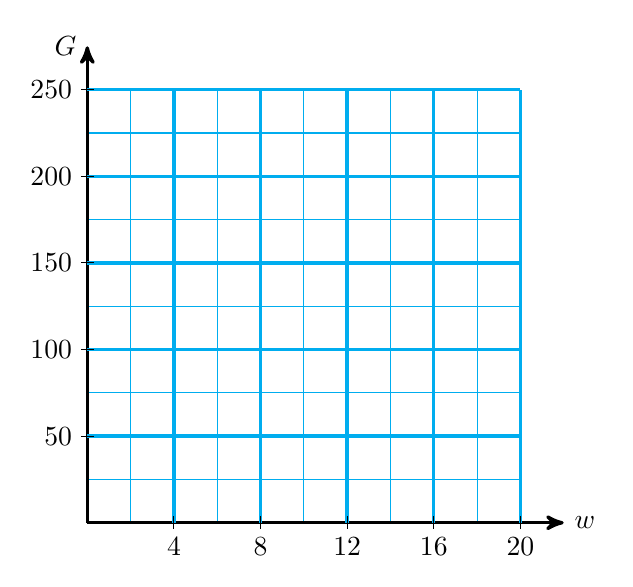
\begin{tikzpicture} [scale=.55]
\coordinate (O) at (0,0);
\draw[cyan] (O) grid (10,10);
\draw[black,very thick, ->, >=stealth'] (O)--(11.,0) node[right]{$w$};
\draw[black,very thick, ->, >=stealth'] (O)--(0,11.) node[left]{$G$};
\foreach \x [evaluate=\x as \xi using int(2*\x] in  {2,4,6,8,10} {
 \draw[cyan, very thick] (\x,0) --++(0,10);
 \draw[black] (\x,.15) --++(0,-.3) node[below, yshift=-2, fill=white, inner sep=1]   {$\xi$};
}
\foreach \x [evaluate=\x as \xi using int(25*\x] in  {2,4,6,8,10} {
 \draw[cyan, very thick] (0,\x) --++(10,0);
 \draw[black] (.15,\x) --++(-.3,0) node[left, xshift=-2, fill=white, inner sep=1]   {$\xi$};
}
\end{tikzpicture}
\newline


hp-3-1-21 grid

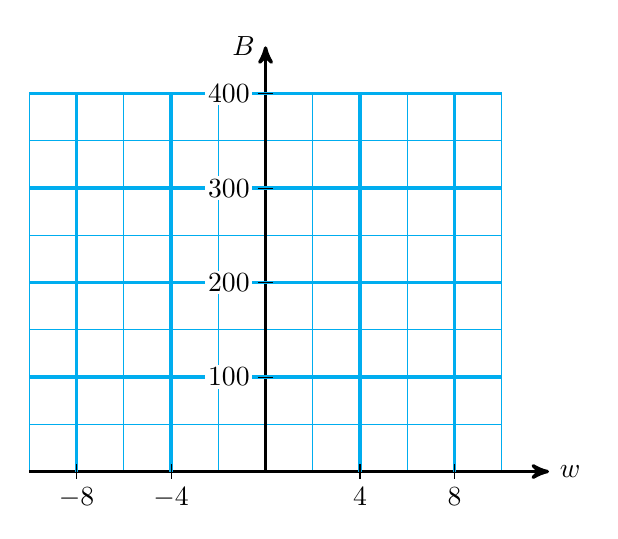
\begin{tikzpicture} [scale=.6]
\coordinate (O) at (0,0);
\draw[cyan] (-5,0) grid (5,8);
\draw[black,very thick, ->, >=stealth'] (-5,0)--(6.,0) node[right]{$w$};
\draw[black,very thick, ->, >=stealth'] (O)--(0,9.) node[left]{$B$};
\foreach \x [evaluate=\x as \xi using int(2*\x] in  {-4,-2,2,4} {
 \draw[cyan, very thick] (\x,0) --++(0,8);
 \draw[black] (\x,.15) --++(0,-.3) node[below, yshift=-2, fill=white, inner sep=1]   {$\xi$};
}
\foreach \x [evaluate=\x as \xi using int(50*\x] in  {2,4,6,8} {
 \draw[cyan, very thick] (-5,\x) --++(10,0);
 \draw[black] (.15,\x) --++(-.3,0) node[left, xshift=-2, fill=white, inner sep=1]   {$\xi$};
}
\end{tikzpicture}
\newline


hp-3-1-21ans

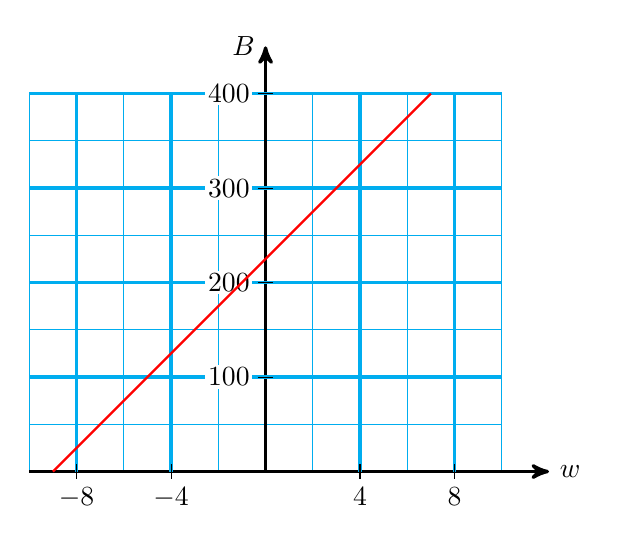
\begin{tikzpicture} [scale=.6]
\coordinate (O) at (0,0);
\draw[cyan] (-5,0) grid (5,8);
\draw[black,very thick, ->, >=stealth'] (-5,0)--(6.,0) node[right]{$w$};
\draw[black,very thick, ->, >=stealth'] (O)--(0,9.) node[left]{$B$};
\foreach \x [evaluate=\x as \xi using int(2*\x] in  {-4,-2,2,4} {
 \draw[cyan, very thick] (\x,0) --++(0,8);
 \draw[black] (\x,.15) --++(0,-.3) node[below, yshift=-2, fill=white, inner sep=1]   {$\xi$};
}
\foreach \x [evaluate=\x as \xi using int(50*\x] in  {2,4,6,8} {
 \draw[cyan, very thick] (-5,\x) --++(10,0);
 \draw[black] (.15,\x) --++(-.3,0) node[left, xshift=-2, fill=white, inner sep=1]   {$\xi$};
}
\draw[red,thick] (-4.5,0)--(3.5,8);
\end{tikzpicture}
\newline


hp-3-1-22 grid

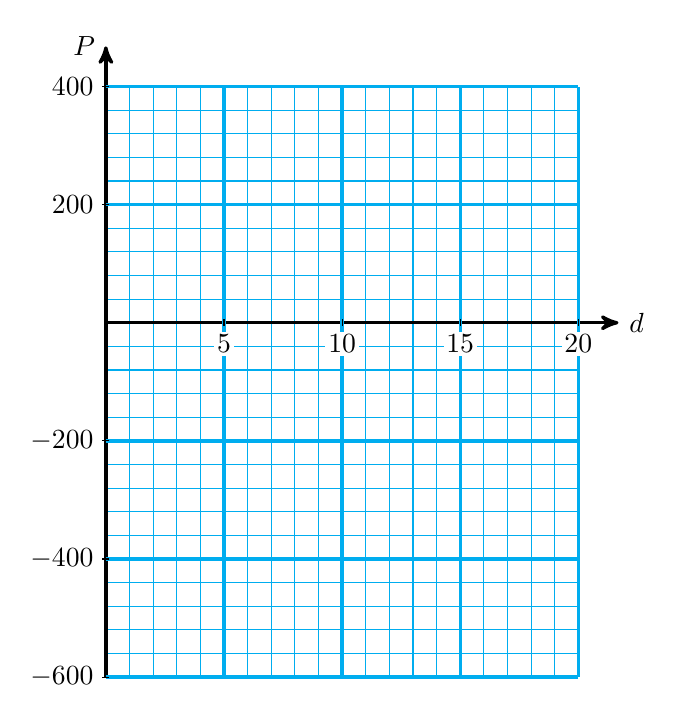
\begin{tikzpicture} [scale=.3]
\draw[cyan] (0,-15) grid (20,10);
\draw[black,very thick, ->, >=stealth'] (0,0)--(21.7,0) node[right]{$d$};
\draw[black,very thick, ->, >=stealth'] (0,-15)--(0,11.7) node[left]{$P$};
\foreach \x in  {5,10,15,20} {
 \draw[cyan, very thick] (\x,-15) --++(0,25);
 \draw[black] (\x,.15) --++(0,-.3) node[below, yshift=-2, fill=white, inner sep=1]   {$\x$};
}
\foreach \x [evaluate=\x as \xi using int(40*\x] in  {-15,-10,-5,5,10} {
 \draw[cyan, very thick] (0,\x) --++(20,0);
 \draw[black] (.15,\x) --++(-.3,0) node[left, xshift=-2, fill=white, inner sep=1]   {$\xi$};
}
\end{tikzpicture}
\newline

\section{Chap 3 Section 2}


fig-3-2-1 cross multiply

        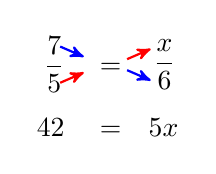
\begin{tikzpicture}
        \coordinate (O) at (0,0);
        \def\dx{.3};
        \def\dy{.13};
        \coordinate (A) at (\dx,-\dy);
        \coordinate (B) at (\dx,\dy);
        \node[left] at (O) {$\displaystyle{\frac{7}{5}}\quad={}$};
        \node[right] at (O) {$\,\displaystyle{\frac{x}{6}}$};
        \draw[blue,thick,->,>=stealth'] (-0.7,0.1)++(-\dx,\dy)--++(A);
        \draw[blue,thick,->,>=stealth'] (0.15,-0.2)++(-\dx,\dy)--++(A);
        \draw[red,thick,->,>=stealth'] (-0.7, -0.1)++(-\dx,-\dy)--++(B);
        \draw[red,thick,->,>=stealth'] (0.15,0.2)++(-\dx,-\dy)--++(B);
        \node[left] at (0,-.8) {$42\quad={}$};
        \node[right] at (0,-.8) {$5x$};
\end{tikzpicture}
\newline


fig-3-2-2 grid

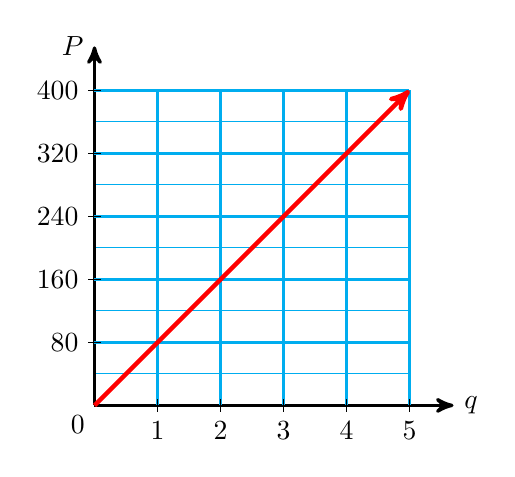
\begin{tikzpicture} [scale=.8]
\coordinate (O) at (0,0);
\draw[cyan] (O) grid[ystep=1/2] (5,5);
\draw[black,very thick, ->, >=stealth'] (O)--(5.7,0) node[right]{$q$};
\draw[black,very thick, ->, >=stealth'] (O)--(0,5.7) node[left]{$P$};
\foreach \x in  {1,2,3,4,5} {
 \draw[cyan, very thick] (\x, 0) --++(0,5);
 \draw[black] (\x,.1) --++(0,-.2) node[below]   {$\x$};
}
\foreach \x [evaluate=\x as \xi using int(80*\x] in  {1,2,3,4,5} {
 \draw[cyan, very thick] (0,\x) --++(5,0);
 \draw[black] (.1,\x) --++(-.2,0) node[left]   {$\xi$};
}
\node[below left] at (O) {$0$};
\draw[red,ultra thick, ->, >=stealth'] (O)--(5,5);
\end{tikzpicture}
\newline


hp-3-2-23 grid

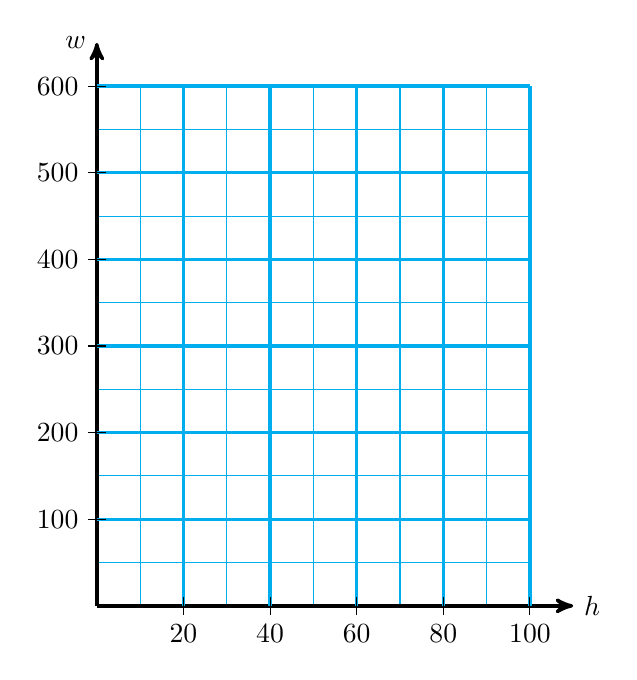
\begin{tikzpicture} [scale=1.1]
\coordinate (O) at (0,0);
\draw[cyan] (O) grid[step=1/2] (5,6);
\draw[black,very thick, ->, >=stealth'] (O)--(5.5,0) node[right]{$h$};
\draw[black,very thick, ->, >=stealth'] (O)--(0,6.5) node[left]{$w$};
\foreach \x [evaluate=\x as \xi using int(20*\x] in  {1,2,3,4,5} {
 \draw[cyan, very thick] (\x, 0) --++(0,6);
 \draw[black] (\x,.1) --++(0,-.2) node[below]   {$\xi$};
}
\foreach \x [evaluate=\x as \xi using int(100*\x] in  {1,2,3,4,5,6} {
 \draw[cyan, very thick] (0,\x) --++(5,0);
 \draw[black] (.1,\x) --++(-.2,0) node[left]   {$\xi$};
}
\end{tikzpicture}
\newline


hp-3-2-23ans

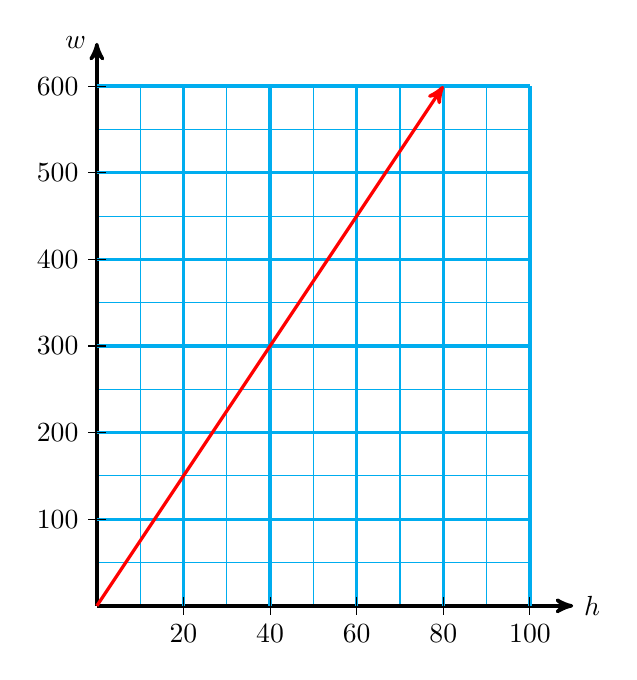
\begin{tikzpicture} [scale=1.1]
\coordinate (O) at (0,0);
\draw[cyan] (O) grid[step=1/2] (5,6);
\draw[black,very thick, ->, >=stealth'] (O)--(5.5,0) node[right]{$h$};
\draw[black,very thick, ->, >=stealth'] (O)--(0,6.5) node[left]{$w$};
\foreach \x [evaluate=\x as \xi using int(20*\x] in  {1,2,3,4,5} {
 \draw[cyan, very thick] (\x, 0) --++(0,6);
 \draw[black] (\x,.1) --++(0,-.2) node[below]   {$\xi$};
}
\foreach \x [evaluate=\x as \xi using int(100*\x] in  {1,2,3,4,5,6} {
 \draw[cyan, very thick] (0,\x) --++(5,0);
 \draw[black] (.1,\x) --++(-.2,0) node[left]   {$\xi$};
}
\draw[red,very thick, ->, >=stealth'] (0,0)--(4,6);
\end{tikzpicture}
\newline


hp-3-2-24 grid

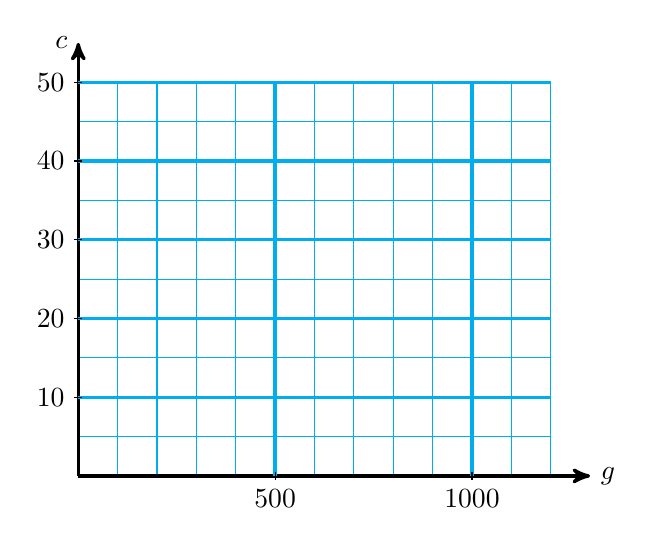
\begin{tikzpicture} [scale=.5]
\coordinate (O) at (0,0);
\draw[cyan] (O) grid (12,10);
\draw[black,very thick, ->, >=stealth'] (O)--(13,0) node[right]{$g$};
\draw[black,very thick, ->, >=stealth'] (O)--(0,11) node[left]{$c$};
\foreach \x [evaluate=\x as \xi using int(100*\x] in  {5,10} {
 \draw[cyan, very thick] (\x, 0) --++(0,10);
 \draw[black] (\x,.1) --++(0,-.2) node[below]   {$\xi$};
}
\foreach \x [evaluate=\x as \xi using int(5*\x] in  {2,4,6,8,10} {
 \draw[cyan, very thick] (0,\x) --++(12,0);
 \draw[black] (.1,\x) --++(-.2,0) node[left]   {$\xi$};
}
\end{tikzpicture}
\newline


hp-3-2-26 grid

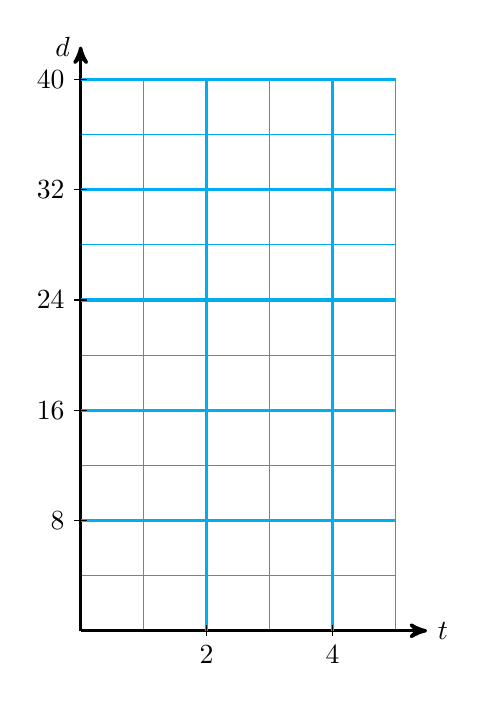
\begin{tikzpicture} [xscale=.8, yscale=.7]
\coordinate (O) at (0,0);
\draw[cyan] (O) grid (5,10);
\draw[black,very thick, ->, >=stealth'] (O)--(5.5,0) node[right]{$t$};
\draw[black,very thick, ->, >=stealth'] (O)--(0,10.6) node[left]{$d$};
\foreach \x in  {2,4} {
 \draw[cyan, very thick] (\x, 0) --++(0,10);
 \draw[black] (\x,.1) --++(0,-.2) node[below]   {$\x$};
}
\foreach \x [evaluate=\x as \xi using int(4*\x] in  {2,4,6,8,10} {
 \draw[cyan, very thick] (0,\x) --++(5,0);
 \draw[black] (.1,\x) --++(-.2,0) node[left]   {$\xi$};
}
\end{tikzpicture}
\newline


hp-3-2-27 grid

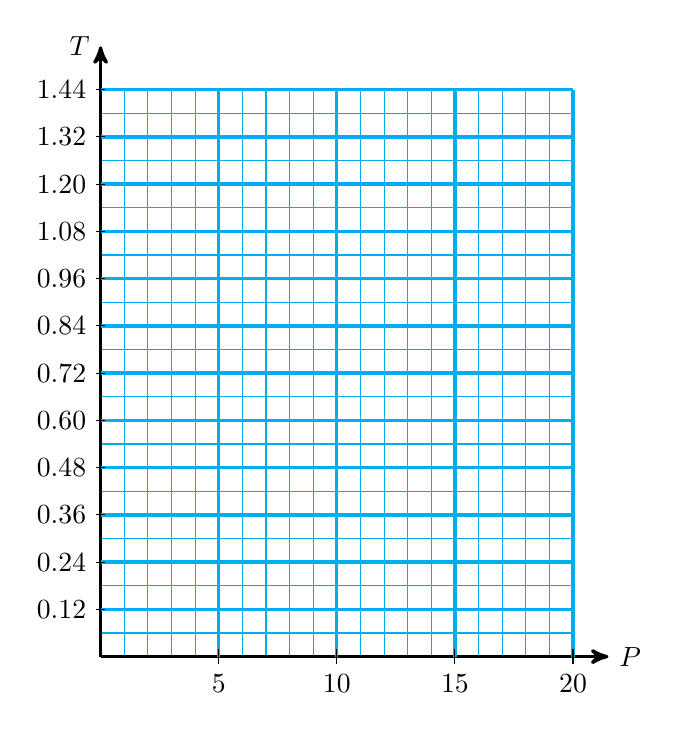
\begin{tikzpicture} [xscale=.3, yscale=5]
\coordinate (O) at (0,0);
\draw[cyan] (O) grid[ystep=3/50] (20,1.44);
\draw[black,very thick, ->, >=stealth'] (O)--(21.5,0) node[right]{$P$};
\draw[black,very thick, ->, >=stealth'] (O)--(0,1.55) node[left]{$T$};
\foreach \x in  {5,10,15,20} {
 \draw[cyan, very thick] (\x, 0) --++(0,1.44);
 \draw[black] (\x,.02) --++(0,-.04) node[below]   {$\x$};
}
\foreach \x in  {0.12,0.24,0.36,0.48,0.60,0.72,0.84,0.96,1.08,1.20,1.32,1.44} {
 \draw[cyan, very thick] (0,\x) --++(20,0);
 \draw[black] (.2,\x) --++(-.4,0) node[left,style={/pgf/number format/.cd,fixed,precision=2}] {$\x$};
}
\end{tikzpicture}
\newline


hp-3-2-27ans

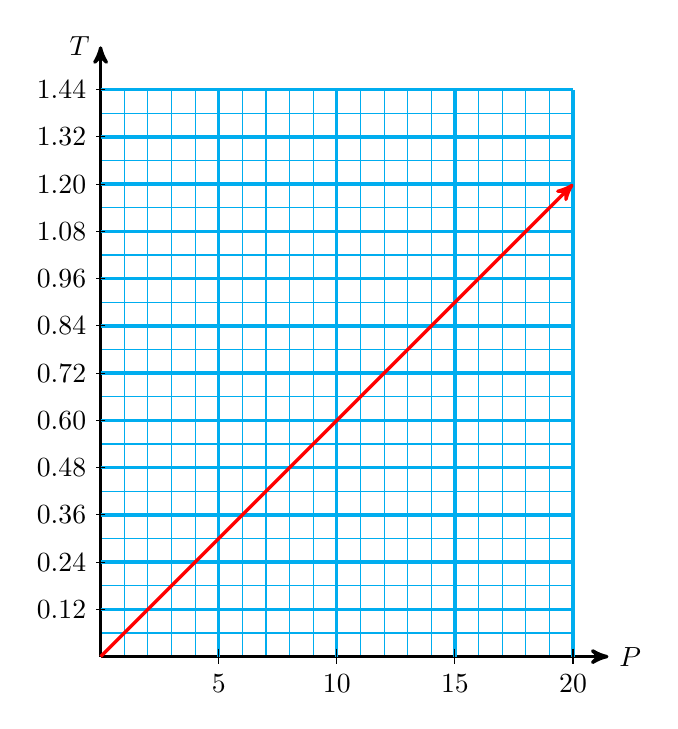
\begin{tikzpicture} [xscale=.3, yscale=5]
\coordinate (O) at (0,0);
\draw[cyan] (O) grid[ystep=3/50] (20,1.44);
\draw[black,very thick, ->, >=stealth'] (O)--(21.5,0) node[right]{$P$};
\draw[black,very thick, ->, >=stealth'] (O)--(0,1.55) node[left]{$T$};
\foreach \x in  {5,10,15,20} {
 \draw[cyan, very thick] (\x, 0) --++(0,1.44);
 \draw[black] (\x,.02) --++(0,-.04) node[below]   {$\x$};
}
\foreach \x in  {0.12,0.24,0.36,0.48,0.60,0.72,0.84,0.96,1.08,1.20,1.32,1.44} {
 \draw[cyan, very thick] (0,\x) --++(20,0);
 \draw[black] (.2,\x) --++(-.4,0) node[left,style={/pgf/number format/.cd,fixed,precision=2}] {$\x$};
}
\draw[red, very thick, ->, >=stealth'] (0,0)--(20, 1.2);
\end{tikzpicture}
\newline


hp-3-2-29 grid

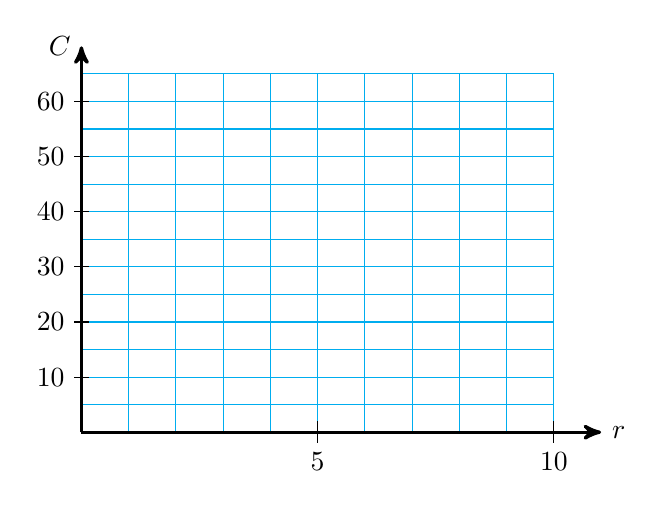
\begin{tikzpicture} [xscale=.6, yscale=0.07]
\coordinate (O) at (0,0);
\draw[cyan] (O) grid[ystep=5] (10,65);
\draw[black,very thick, ->, >=stealth'] (O)--(11,0) node[right]{$r$};
\draw[black,very thick, ->, >=stealth'] (O)--(0,70) node[left]{$C$};
\foreach \x in  {5,10} {
% \draw[cyan, very thick] (\x, 0) --++(0,65);
 \draw[black] (\x,2) --++(0,-4) node[below]   {$\x$};
}
\foreach \x in  {10,20,...,60} {
% \draw[cyan, very thick] (0,\x) --++(10,0);
 \draw[black] (.15,\x) --++(-.3,0) node[left,style={/pgf/number format/.cd,fixed,precision=2}] {$\x$};
}
\end{tikzpicture}
\newline


hp-3-2-29ans

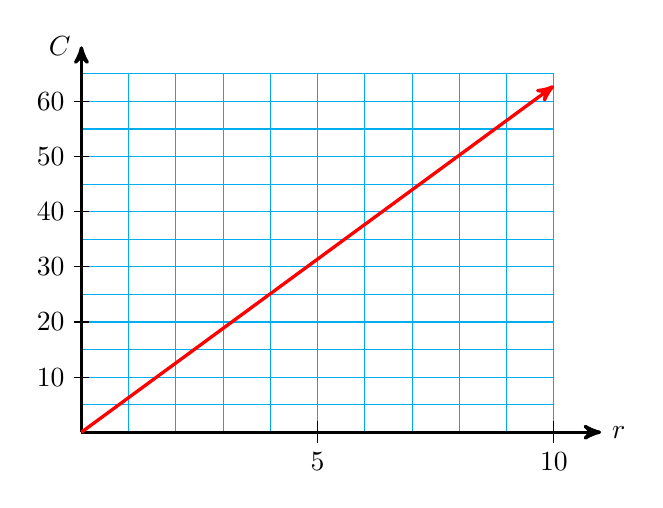
\begin{tikzpicture} [xscale=.6, yscale=0.07]
\coordinate (O) at (0,0);
\draw[cyan] (O) grid[ystep=5] (10,65);
\draw[black,very thick, ->, >=stealth'] (O)--(11,0) node[right]{$r$};
\draw[black,very thick, ->, >=stealth'] (O)--(0,70) node[left]{$C$};
\foreach \x in  {5,10} {
% \draw[cyan, very thick] (\x, 0) --++(0,65);
 \draw[black] (\x,2) --++(0,-4) node[below]   {$\x$};
}
\foreach \x in  {10,20,...,60} {
% \draw[cyan, very thick] (0,\x) --++(10,0);
 \draw[black] (.15,\x) --++(-.3,0) node[left,style={/pgf/number format/.cd,fixed,precision=2}] {$\x$};
}
\draw[red, very thick, ->, >=stealth'] (0,0)--(10, 20*pi);
\end{tikzpicture}
\newline


hp-3-2-30 grid

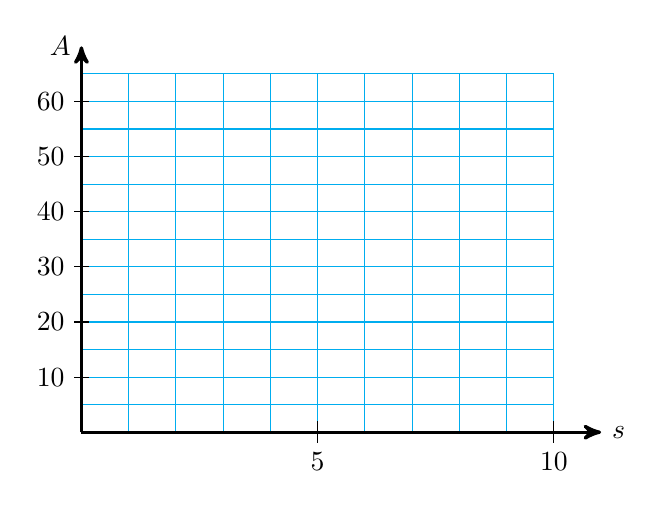
\begin{tikzpicture} [xscale=.6, yscale=0.07]
\coordinate (O) at (0,0);
\draw[cyan] (O) grid[ystep=5] (10,65);
\draw[black,very thick, ->, >=stealth'] (O)--(11,0) node[right]{$s$};
\draw[black,very thick, ->, >=stealth'] (O)--(0,70) node[left]{$A$};
\foreach \x in  {5,10} {
% \draw[cyan, very thick] (\x, 0) --++(0,65);
 \draw[black] (\x,2) --++(0,-4) node[below]   {$\x$};
}
\foreach \x in  {10,20,...,60} {
% \draw[cyan, very thick] (0,\x) --++(10,0);
 \draw[black] (.15,\x) --++(-.3,0) node[left,style={/pgf/number format/.cd,fixed,precision=2}] {$\x$};
}
\end{tikzpicture}
\newline

\section{Chap 3 Section 3}




fig-3-3-ex1 graph 

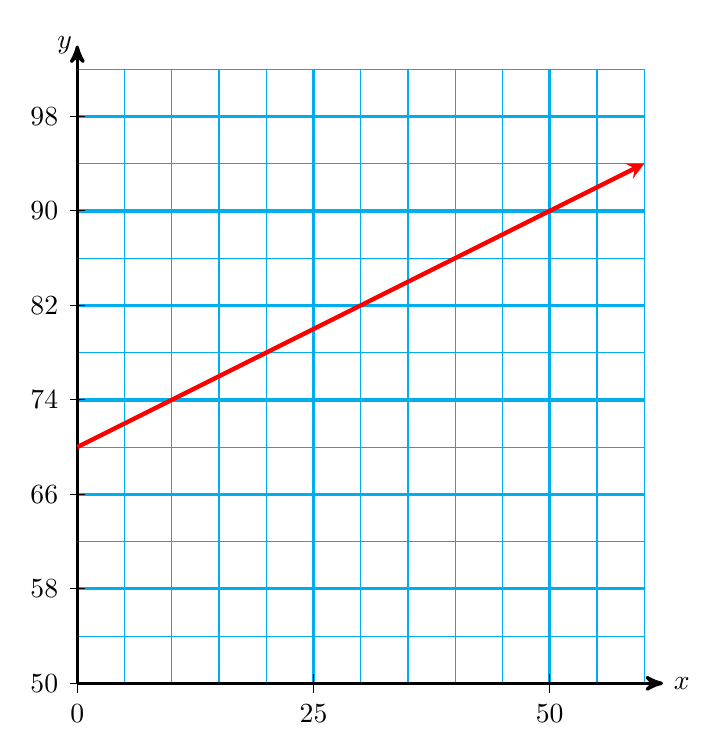
\begin{tikzpicture} [xscale=.12, yscale=.15]
\coordinate (O) at (0,0);
\draw[cyan] (O) grid[xstep=5, ystep=4] (60,52);
\foreach \x  in  {0,25, 50} {
 \draw[cyan, very thick] (\x,0) --++(0,52);
 \draw[black] (\x,0.8) --++(0,-1.6) node[below, yshift=-3, fill=white, inner sep=1]   {$\x$};
}
\foreach \x [evaluate=\x as \xi using int(\x+50] in  {0, 8, ..., 48} {
 \draw[cyan, very thick] (0,\x) --++(60,0);
 \draw[black] (.8,\x) --++(-1.6,0) node[left, xshift=-3, fill=white, inner sep=1]   {$\xi$};
}
\draw[black,very thick, ->, >=stealth'] (O)--++(62,0) node[right]{$x$};
\draw[black,very thick, ->, >=stealth'] (O)--++(0,54) node[left, xshift=2]{$y$};
\draw[red, ultra thick, ->,>=stealth] (0,20)--++(60,24);
\end{tikzpicture}
\newline



fig-3-3-1 graph 

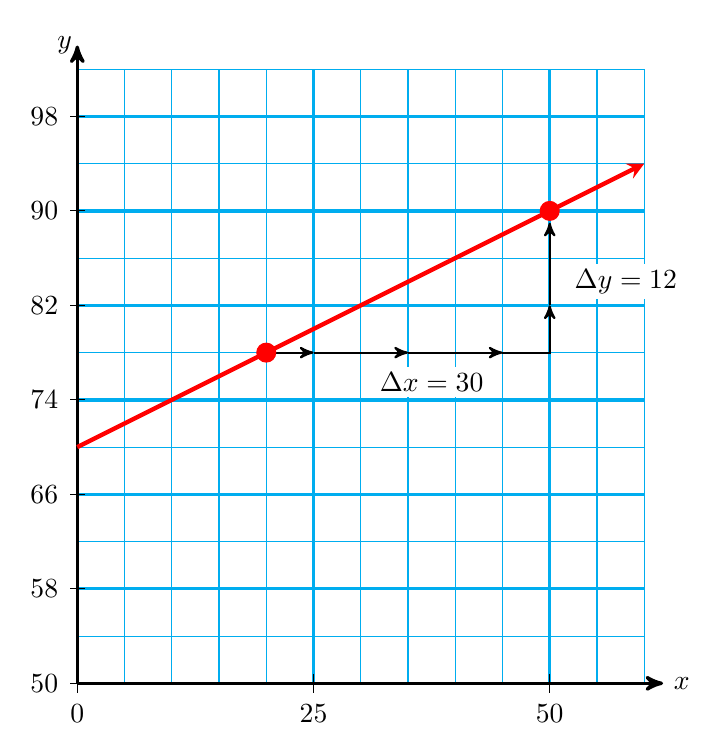
\begin{tikzpicture} [xscale=.12, yscale=.15]
\coordinate (O) at (0,0);
\draw[cyan] (O) grid[xstep=5, ystep=4] (60,52);
\foreach \x  in  {0,25, 50} {
 \draw[cyan, very thick] (\x,0) --++(0,52);
 \draw[black] (\x,0.8) --++(0,-1.6) node[below, yshift=-3, fill=white, inner sep=1]   {$\x$};
}
\foreach \x [evaluate=\x as \xi using int(\x+50] in  {0, 8, ..., 48} {
 \draw[cyan, very thick] (0,\x) --++(60,0);
 \draw[black] (.8,\x) --++(-1.6,0) node[left, xshift=-3, fill=white, inner sep=1]   {$\xi$};
}
\draw[black,very thick, ->, >=stealth'] (O)--++(62,0) node[right]{$x$};
\draw[black,very thick, ->, >=stealth'] (O)--++(0,54) node[left, xshift=2]{$y$};
\draw[red, ultra thick, ->,>=stealth] (0,20)--++(60,24);
\draw[black,thick,->,>=stealth'] (20,28)--++(5,0);
\draw[black,thick,->,>=stealth'] (25,28)--++(10,0);
\draw[black,thick,->,>=stealth'] (35,28)--++(10,0);
\draw[black,thick,->,>=stealth'] (45,28)--++(5,0)--++(0,4);
\draw[black,thick,->,>=stealth'] (50,32)--++(0,7);
\filldraw[red] (20,28) ellipse (1cm and 0.8cm);
\filldraw[red] (50,40) ellipse (1cm and 0.8cm);
\node[text=black,fill=white, inner sep=2] at (37.5,25.5) {$\Delta x = 30$};
\node[right,text=black,fill=white, inner sep=2] at (52,34) {$\Delta y = 12$};
\end{tikzpicture}
\newline



fig-3-3-ex2 slope

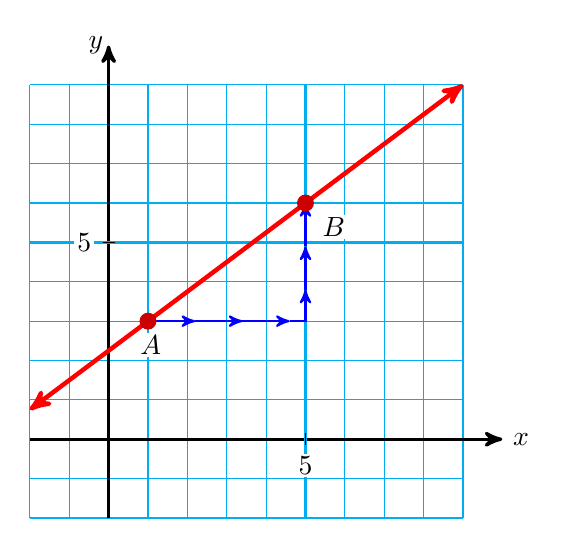
\begin{tikzpicture} [scale=.5]
\coordinate (O) at (0,0);
\draw[cyan] (-2,-2) grid (9,9);
\draw[black,very thick, ->, >=stealth'] (-2,0)--(10,0) node[right]{$x$};
\draw[black,very thick, ->, >=stealth'] (0,-2)--(0,10) node[left, xshift=2]{$y$};
\foreach \x  in  {5} {
 \draw[cyan, very thick] (\x,-2) --++(0,11);
 \draw[cyan, very thick] (-2,\x) --++(11,0);
 \draw[black] (\x,.15) --++(0,-.3) node[below, yshift=-3, fill=white, inner sep=1]   {$\x$};
 \draw[black] (.15,\x) --++(-.3,0) node[left, xshift=-3, fill=white, inner sep=1]   {$\x$};
}
\foreach \x in {1, 2.2, 3.4} 
 \draw[blue,thick, ->, >=stealth'] (\x,3)--++(1.2,0);
\draw[blue,thick, ->, >=stealth'] (4.6,3)--++(0.4,0)--++(0,0.8);
\draw[blue,thick, ->, >=stealth'] (5,3.8)--++(0,1.1);
\draw[blue,thick, ->, >=stealth'] (5,4.9)--++(0,1.1);
\draw[red, ultra thick, <->, >=stealth'] (-2,3/4)--(9,9);
\filldraw[red!80!black] (1,3) circle (2mm) node[text=black,below,yshift=-4, xshift=1, fill=white, inner sep=1] {$A$};
\filldraw[red!80!black] (5,6) circle (2mm) node[text=black,below right,yshift=-4, xshift=5, fill=white, inner sep=1] {$B$};
\end{tikzpicture}
\newline



fig-3-3-ex3 speed as slope

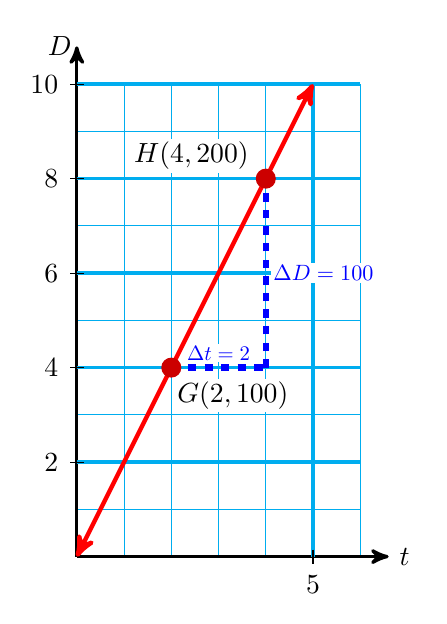
\begin{tikzpicture} [scale=.6]
\coordinate (O) at (0,0);
\draw[cyan] (O) grid (6,10);
\draw[black,very thick, ->, >=stealth'] (O)--(6.6,0) node[right]{$t$};
\draw[black,very thick, ->, >=stealth'] (O)--(0,10.8) node[left, xshift=2]{$D$};
\foreach \x  in  {5} {
 \draw[cyan, very thick] (\x,0) --++(0,10);
 \draw[black] (\x,.15) --++(0,-.3) node[below, yshift=-3, fill=white, inner sep=1]   {$\x$};
}
\foreach \x [evaluate=\x as \xi using int(25*\x] in  {2,4,6,8,10} {
 \draw[cyan, very thick] (0,\x) --++(6,0);
 \draw[black] (.15,\x) --++(-.3,0) node[left, xshift=-3, fill=white, inner sep=1]   {$\x$};
}
\draw[blue, line width=0.8mm, dashed] (2,4)--++(2,0) node[above,midway, yshift=1, midway, fill=white, inner sep=1, scale=.75] {$\Delta t = 2$};
\draw[blue, line width=0.8mm, dashed] (4,4)--++(0,4) node[right,midway, xshift=1, midway, fill=white, inner sep=1, scale=.8] {$\Delta D = 100$};
\draw[red, ultra thick, <->, >=stealth'] (O)--(5,10);
\filldraw[red!80!black] (2,4) circle (2mm) node[text=black,below right,yshift=-4, xshift=1, fill=white, inner sep=1] {$G(2,100)$};
\filldraw[red!80!black] (4,8) circle (2mm) node[text=black,above left,yshift=2, xshift=-5, fill=white, inner sep=1] {$H(4,200)$};
\end{tikzpicture}
\newline


fig-3-3-2a

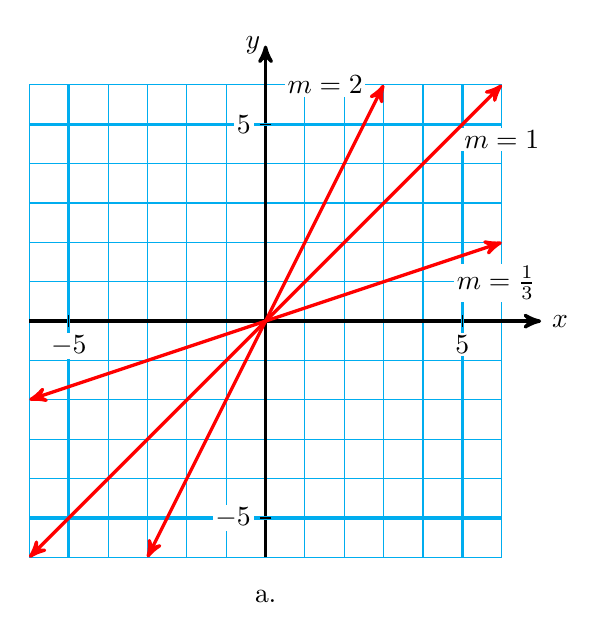
\begin{tikzpicture} [scale=.5]
\coordinate (O) at (0,0);
\draw[cyan] (-6,-6) grid (6,6);
\draw[black,very thick, ->, >=stealth'] (-6,0)--(7.,0) node[right]{$x$};
\draw[black,very thick, ->, >=stealth'] (0,-6)--(0,7.) node[left, xshift=2]{$y$};
\foreach \x  in  {-5, 5} {
 \draw[cyan, very thick] (\x,-6) --++(0,12);
 \draw[cyan, very thick] (-6,\x) --++(12,0);
 \draw[black] (\x,.15) --++(0,-.3) node[below, yshift=-2, fill=white, inner sep=1]   {$\x$};
 \draw[black] (.15,\x) --++(-.3,0) node[left, xshift=-2, fill=white, inner sep=1]   {$\x$};
}
\draw[red, very thick, <->, >=stealth'] (-3,-6)--(3,6) node[left, xshift=-6, text=black, fill=white, inner sep=1] {$m=2$};
\draw[red, very thick, <->, >=stealth'] (-6,-6)--(6,6) node[below, yshift=-.52cm, text=black, fill=white, inner sep=1] {$m=1$};
\draw[red, very thick, <->, >=stealth'] (-6,-2)--(6,2) node[below, xshift=-2, yshift=-.25cm, text=black, fill=white, inner sep=1] {$m=\frac{1}{3}$};
\node at (0,-7){a.};
\end{tikzpicture}
\newline


fig-3-3-2b

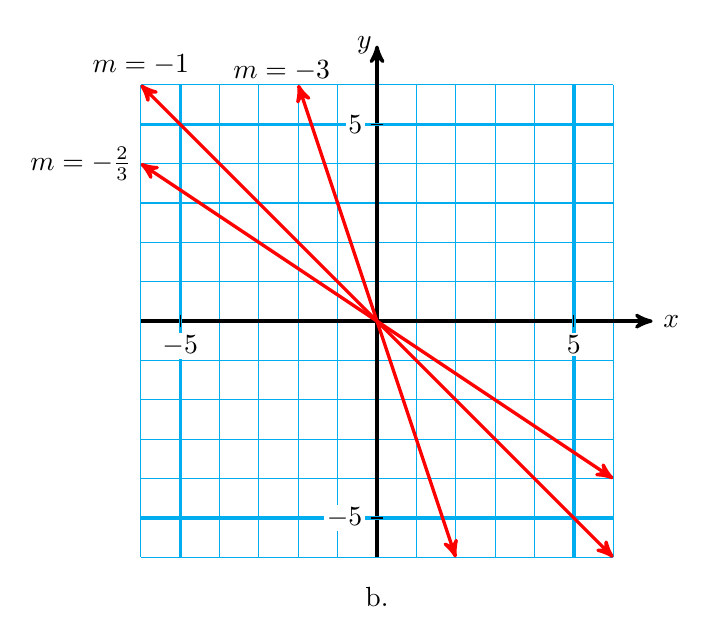
\begin{tikzpicture} [scale=.5]
\coordinate (O) at (0,0);
\draw[cyan] (-6,-6) grid (6,6);
\draw[black,very thick, ->, >=stealth'] (-6,0)--(7.,0) node[right]{$x$};
\draw[black,very thick, ->, >=stealth'] (0,-6)--(0,7.) node[left, xshift=2]{$y$};
\foreach \x  in  {-5, 5} {
 \draw[cyan, very thick] (\x,-6) --++(0,12);
 \draw[cyan, very thick] (-6,\x) --++(12,0);
 \draw[black] (\x,.15) --++(0,-.3) node[below, yshift=-2, fill=white, inner sep=1]   {$\x$};
 \draw[black] (.15,\x) --++(-.3,0) node[left, xshift=-2, fill=white, inner sep=1]   {$\x$};
}
\draw[red, very thick, <->, >=stealth'] (2,-6)--(-2,6) node[above, xshift=-6, text=black, fill=white, inner sep=1] {$m=-3$};
\draw[red, very thick, <->, >=stealth'] (6,-6)--(-6,6) node[above, yshift=2, text=black, fill=white, inner sep=1] {$m=-1$};
\draw[red, very thick, <->, >=stealth'] (6,-4)--(-6,4) node[left, xshift=-2,  text=black, fill=white, inner sep=1] {$m=-\frac{2}{3}$};
\node at (0,-7){b.};
\end{tikzpicture}
\newline


hp-3-3-1

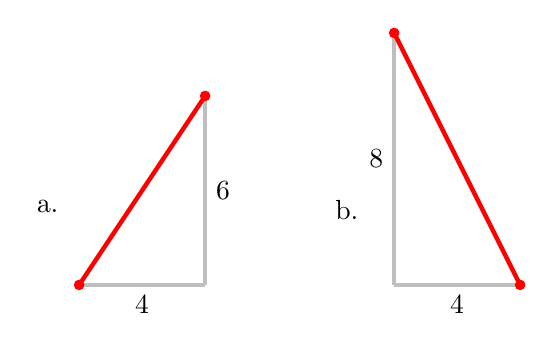
\begin{tikzpicture} [scale=.4]
\coordinate (O) at (0,0);
\coordinate (A) at ($ (O)+(4,6) $);
\draw[lightgray,very thick] (O)--++(4,0) node[below,midway, text=black] {4};
\draw[lightgray,very thick] (A)--++(0,-6) node[right,midway, text=black] {6};
\filldraw[red] (O) circle (1.5mm);
\filldraw[red] (A) circle (1.5mm);
\draw[red,ultra thick] (O)--(A);
\node[below] at ($ (O)+(-1,3) $) {a.};

\coordinate (O) at (14,0);
\coordinate (A) at ($ (O)+(-4,8) $);
\draw[lightgray,very thick] (O)--++(-4,0) node[below,midway, text=black] {4};
\draw[lightgray,very thick] (A)--++(0,-8) node[left,midway, text=black] {8};
\filldraw[red] (O) circle (1.5mm);
\filldraw[red] (A) circle (1.5mm);
\draw[red,ultra thick] (O)--(A);
\node[below] at ($ (O)+(-5.5,3) $) {b.};
\end{tikzpicture}
\newline


hp-3-3-2

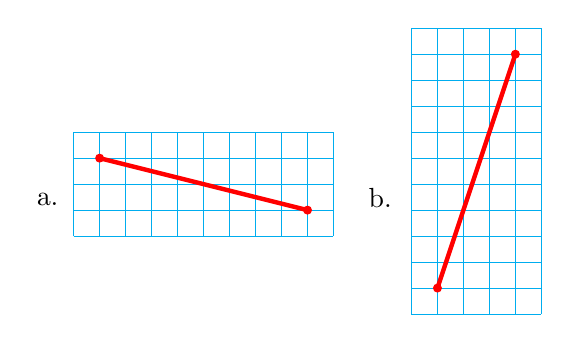
\begin{tikzpicture} [scale=.33]
\coordinate (O) at (0,0);
\coordinate (A) at (1,3);
\coordinate (B) at (9,1);
\draw[cyan] (O) grid ($ (O)+(10,4) $);
\filldraw[red] (B) circle (1.5mm);
\filldraw[red] (A) circle (1.5mm);
\draw[red,ultra thick] (B)--(A);
\node[below] at ($ (O)+(-1,2) $) {a.};

\coordinate (O) at (13,2);
\coordinate (A) at ($ (O)+(1,-4) $);
\coordinate (B) at ($ (O)+(4,5) $);
\draw[cyan] (13,-3) grid (18,8);
\filldraw[red] (B) circle (1.5mm);
\filldraw[red] (A) circle (1.5mm);
\draw[red,ultra thick] (B)--(A);
\node[below] at ($ (O)+(-1.2,0.2) $) {b.};
\end{tikzpicture}
\newline


hp-3-3-3

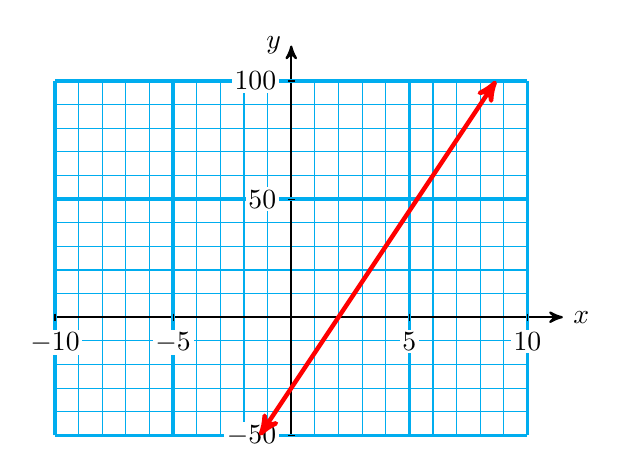
\begin{tikzpicture} [scale=.3]
\draw[cyan] (-10,-5) grid (10,10);
\draw[black, thick,->,>=stealth'] (-10,0)--(11.5,0) node[right]{$x$};
\draw[black, thick,->,>=stealth'] (0,-5)--(0,11.5) node[left]{$y$};
\foreach \x  in  {-10,-5,5,10} {
 \draw[cyan, very thick] (\x,-5) --(\x,10);
 \draw[black] (\x,.15) --++(0,-.3) node[below, yshift=-3, fill=white, inner sep=1]   {$\x$};
}
\foreach \x [evaluate=\x as \xi using int(10*\x] in  {-5,5,10} {
 \draw[cyan, very thick] (-10,\x) --(10,\x);
 \draw[black] (.15,\x) --++(-.3,0) node[left, xshift=-3, fill=white, inner sep=1]   {$\xi$};
}
\draw[red, ultra thick, <->,>=stealth'] (-4/3,-5)--(26/3,10);
\end{tikzpicture}
\newline


hp-3-3-4

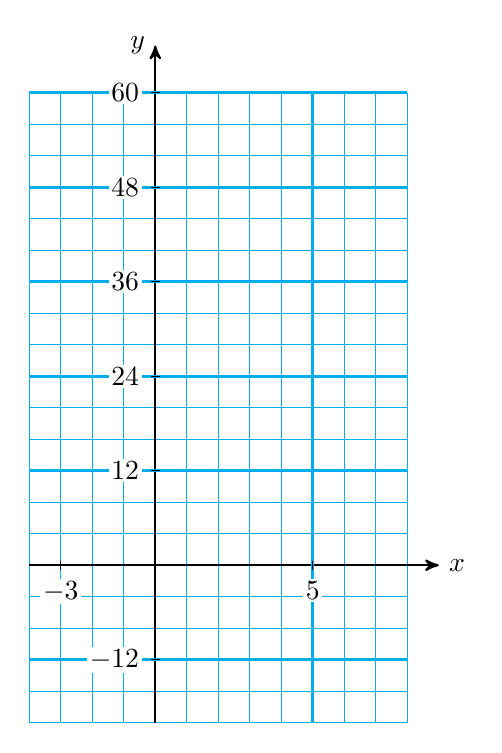
\begin{tikzpicture} [scale=.4]
\draw[cyan] (-4,-5) grid (8,15);
\draw[black, thick,->,>=stealth'] (-4,0)--(9.,0) node[right]{$x$};
\draw[black, thick,->,>=stealth'] (0,-5)--(0,16.5) node[left]{$y$};
\draw[cyan, very thick] (5,-5) --(5,15);
\foreach \x  in  {-3,5} {
 \draw[black] (\x,.15) --++(0,-.3) node[below, yshift=-3, fill=white, inner sep=1]   {$\x$};
}
\foreach \x [evaluate=\x as \xi using int(4*\x] in  {-3,3,6,9,12,15} {
 \draw[cyan, very thick] (-4,\x) --(8,\x);
 \draw[black] (.15,\x) --++(-.3,0) node[left, xshift=-3, fill=white, inner sep=1]   {$\xi$};
}
\end{tikzpicture}
\newline


hp-3-3-5 10-by-10 grid

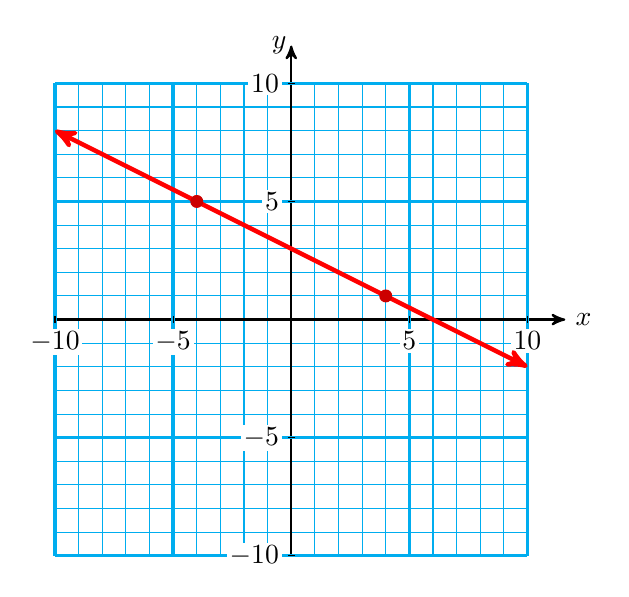
\begin{tikzpicture} [scale=.3]
\coordinate (O) at (0,0);
\draw[cyan] (-10,-10) grid (10,10);
\draw[black,thick, ->, >=stealth'] (-10,0)--(11.6,0) node[right]{$x$};
\draw[black,thick, ->, >=stealth'] (0,-10)--(0,11.6) node[left, xshift=2]{$y$};
\foreach \x in  {-5, 5, -10, 10} {
 \draw[cyan, very thick] (\x,-10) --++(0,20);
 \draw[cyan, very thick] (-10,\x) --++(20,0);
 \draw[black] (\x,.15) --++(0,-.3)  node[below, yshift=-2, fill=white, inner sep=1]   {$\x$};
 \draw[black] (.15,\x) --++(-.3,0)  node[left, xshift=-2, fill=white, inner sep=1]   {$\x$};
}
\draw[red, ultra thick, <->, >=stealth'] (-10,8)--(10,-2);
\filldraw[red!80!black] (-4,5) circle (2.5mm);
\filldraw[red!80!black] (4,1) circle (2.5mm);
\end{tikzpicture}
\newline


hp-3-3-6 10-by-10 grid

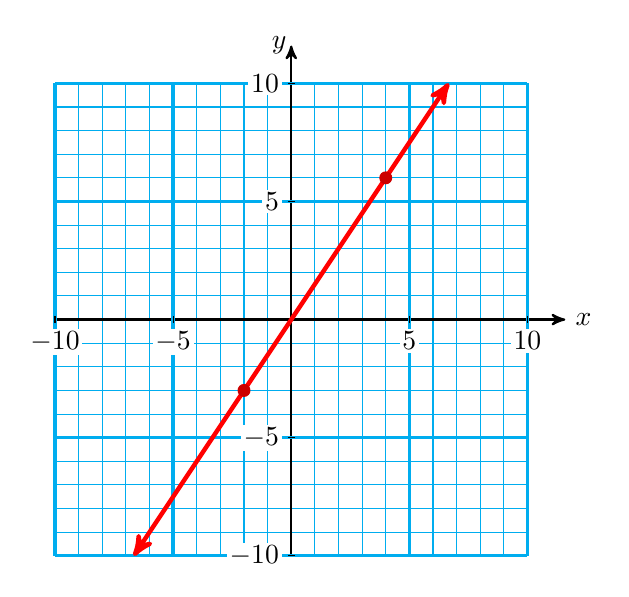
\begin{tikzpicture} [scale=.3]
\coordinate (O) at (0,0);
\draw[cyan] (-10,-10) grid (10,10);
\draw[black,thick, ->, >=stealth'] (-10,0)--(11.6,0) node[right]{$x$};
\draw[black,thick, ->, >=stealth'] (0,-10)--(0,11.6) node[left, xshift=2]{$y$};
\foreach \x in  {-5, 5, -10, 10} {
 \draw[cyan, very thick] (\x,-10) --++(0,20);
 \draw[cyan, very thick] (-10,\x) --++(20,0);
 \draw[black] (\x,.15) --++(0,-.3)  node[below, yshift=-2, fill=white, inner sep=1]   {$\x$};
 \draw[black] (.15,\x) --++(-.3,0)  node[left, xshift=-2, fill=white, inner sep=1]   {$\x$};
}
\draw[red, ultra thick, <->, >=stealth'] (-20/3,-10)--(20/3,10);
\filldraw[red!80!black] (-2,-3) circle (2.5mm);
\filldraw[red!80!black] (4,6) circle (2.5mm);
\end{tikzpicture}
\newline


hp-3-3-7ans 10-by-10 grid

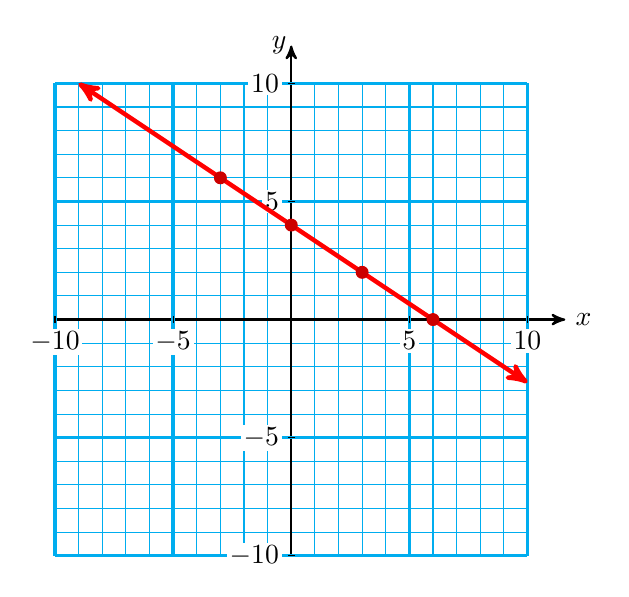
\begin{tikzpicture} [scale=.3]
\coordinate (O) at (0,0);
\draw[cyan] (-10,-10) grid (10,10);
\draw[black,thick, ->, >=stealth'] (-10,0)--(11.6,0) node[right]{$x$};
\draw[black,thick, ->, >=stealth'] (0,-10)--(0,11.6) node[left, xshift=2]{$y$};
\foreach \x in  {-5, 5, -10, 10} {
 \draw[cyan, very thick] (\x,-10) --++(0,20);
 \draw[cyan, very thick] (-10,\x) --++(20,0);
 \draw[black] (\x,.15) --++(0,-.3)  node[below, yshift=-2, fill=white, inner sep=1]   {$\x$};
 \draw[black] (.15,\x) --++(-.3,0)  node[left, xshift=-2, fill=white, inner sep=1]   {$\x$};
}
\draw[red, ultra thick, <->, >=stealth'] (-9,10)--(10,-8/3);
\filldraw[red!80!black] (0,4) circle (2.5mm);
\filldraw[red!80!black] (6,0) circle (2.5mm);
\filldraw[red!80!black] (-3,6) circle (2.5mm);
\filldraw[red!80!black] (3,2) circle (2.5mm);
\end{tikzpicture}
\newline


hp-3-3-9ans 10-by-10 grid

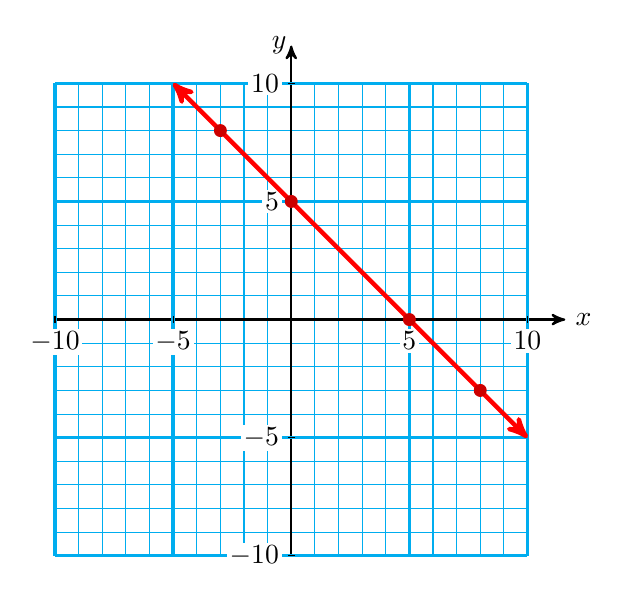
\begin{tikzpicture} [scale=.3]
\coordinate (O) at (0,0);
\draw[cyan] (-10,-10) grid (10,10);
\draw[black,thick, ->, >=stealth'] (-10,0)--(11.6,0) node[right]{$x$};
\draw[black,thick, ->, >=stealth'] (0,-10)--(0,11.6) node[left, xshift=2]{$y$};
\foreach \x in  {-5, 5, -10, 10} {
 \draw[cyan, very thick] (\x,-10) --++(0,20);
 \draw[cyan, very thick] (-10,\x) --++(20,0);
 \draw[black] (\x,.15) --++(0,-.3)  node[below, yshift=-2, fill=white, inner sep=1]   {$\x$};
 \draw[black] (.15,\x) --++(-.3,0)  node[left, xshift=-2, fill=white, inner sep=1]   {$\x$};
}
\draw[red, ultra thick, <->, >=stealth'] (-5,10)--(10,-5);
\filldraw[red!80!black] (0,5) circle (2.5mm);
\filldraw[red!80!black] (5,0) circle (2.5mm);
\filldraw[red!80!black] (-3,8) circle (2.5mm);
\filldraw[red!80!black] (8,-3) circle (2.5mm);
\end{tikzpicture}
\newline


hp-3-3-15 slope

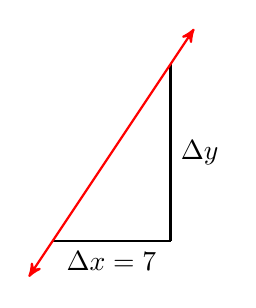
\begin{tikzpicture} [scale=1.5]
\draw[black,thick](0,0)--(1,0) node[below, midway]{$\Delta x=7$};
\draw[black,thick] (1,0)--(1,1.5) node[right, midway]{$\Delta y$};
\draw[red,thick, <->, >=stealth'] (-.2, -.3)--(1.2, 1.8);
\end{tikzpicture}
\newline



hp-3-3-16 slope

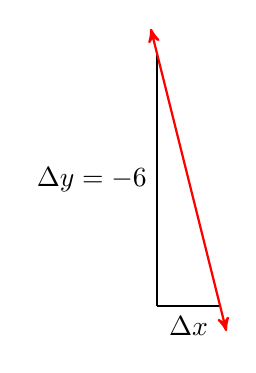
\begin{tikzpicture} [scale=.8]
\draw[black,thick](0,0)--(1,0) node[below, midway]{$\Delta x$};
\draw[black,thick] (0,0)--(0,4) node[left, midway]{$\Delta y=-6$};
\draw[red,thick, <->, >=stealth'] (-.1, 4.4)--(1.1, -.4);
\end{tikzpicture}
\newline


hp-3-3-17

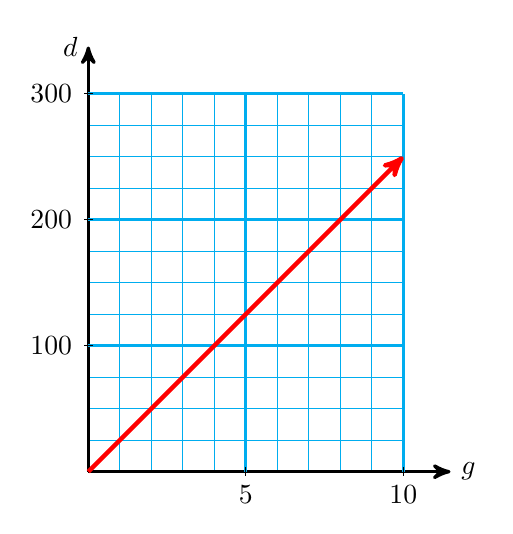
\begin{tikzpicture} [scale=.4]
\coordinate (O) at (0,0);
\draw[cyan] (O) grid (10,12);
\draw[black,very thick, ->, >=stealth'] (O)--(11.5,0) node[right]{$g$};
\draw[black,very thick, ->, >=stealth'] (O)--(0,13.5) node[left]{$d$};
\foreach \x  in  {5,10} {
 \draw[cyan, very thick] (\x,0) --++(0,12);
 \draw[black] (\x,.15) --++(0,-.3) node[below, yshift=-2, fill=white, inner sep=1]   {$\x$};
}
\foreach \x [evaluate=\x as \xi using int(25*\x] in  {4,8,12} {
 \draw[cyan, very thick] (0,\x) --(10,\x);
 \draw[black] (.15,\x) --++(-.3,0) node[left, xshift=-3, fill=white, inner sep=1]   {$\xi$};
}
\draw[red, ultra thick, ->, >=stealth'] (O)--(10,10);
\end{tikzpicture}
\newline


hp-3-3-18

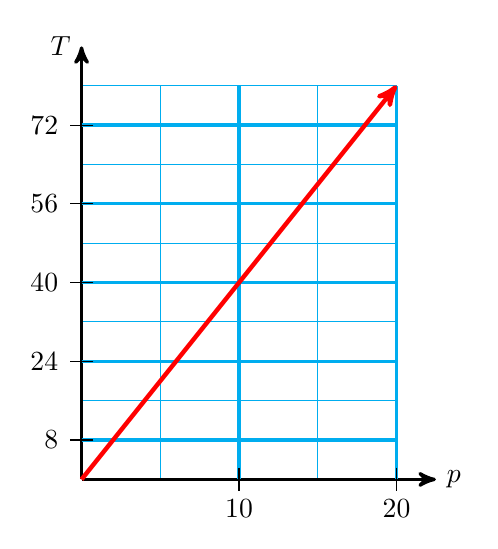
\begin{tikzpicture}
\coordinate (O) at (0,0);
\draw[cyan] (O) grid[ystep=1/2] (4,5);
\draw[black,very thick, ->, >=stealth'] (O)--(4.5,0) node[right]{$p$};
\draw[black,very thick, ->, >=stealth'] (O)--(0,5.5) node[left]{$T$};
\foreach \x [evaluate=\x as \xi using int(5*\x] in  {2,4} {
 \draw[cyan, very thick] (\x,0) --++(0,5);
 \draw[black] (\x,.15) --++(0,-.3) node[below, yshift=-2, fill=white, inner sep=1]   {$\xi$};
}
\foreach \x [evaluate=\x as \xi using int(16*\x] in  {.5,1.5,2.5,3.5,4.5} {
 \draw[cyan, very thick] (0,\x) --(4,\x);
 \draw[black] (.15,\x) --++(-.3,0) node[left, xshift=-3, fill=white, inner sep=1]   {$\xi$};
}
\draw[red, ultra thick, ->, >=stealth'] (O)--(4,5);
\end{tikzpicture}
\newline


hp-3-3-19

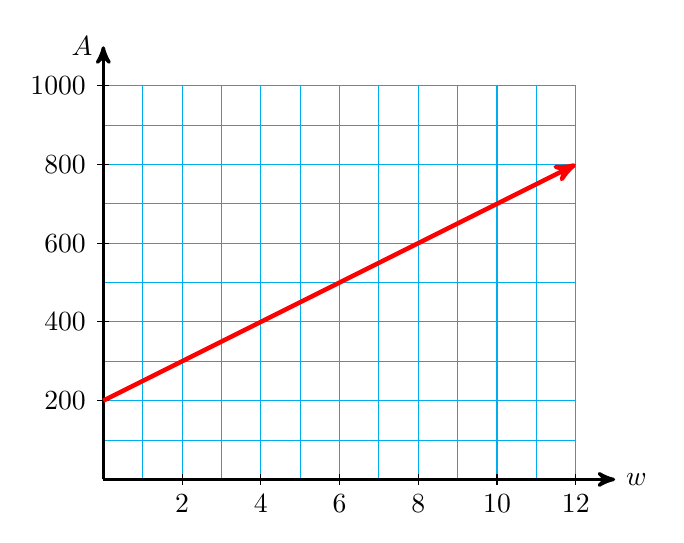
\begin{tikzpicture} [scale=.5]
\coordinate (O) at (0,0);
\draw[cyan] (O) grid (12,10);
\draw[black,very thick, ->, >=stealth'] (O)--(13,0) node[right]{$w$};
\draw[black,very thick, ->, >=stealth'] (O)--(0,11) node[left]{$A$};
\foreach \x in  {2,4,...,12} {
 \draw[black] (\x,.15) --++(0,-.3) node[below, yshift=-2, fill=white, inner sep=1]   {$\x$};
}
\foreach \x [evaluate=\x as \xi using int(100*\x] in  {2,4,...,10} {
 \draw[black] (.15,\x) --++(-.3,0) node[left, xshift=-3, fill=white, inner sep=1]   {$\xi$};
}
\draw[red, ultra thick, ->, >=stealth'] (0,2)--(12,8);
\end{tikzpicture}
\newline


hp-3-3-20

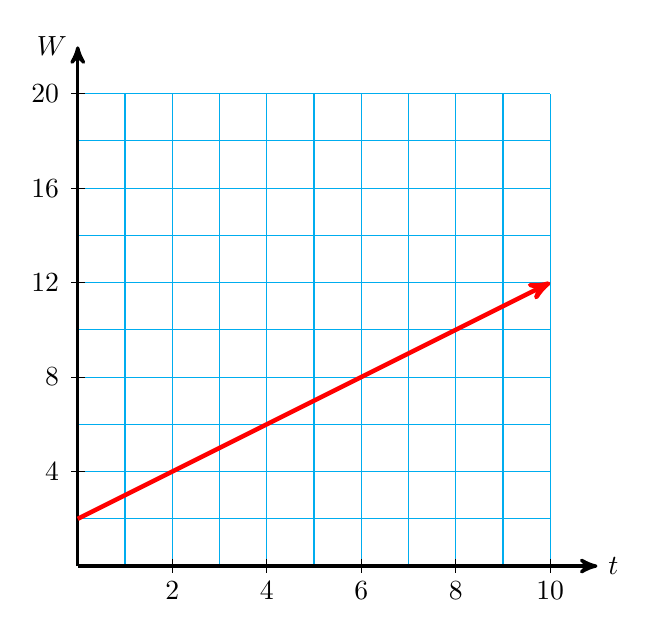
\begin{tikzpicture} [scale=.6]
\coordinate (O) at (0,0);
\draw[cyan] (O) grid (10,10);
\draw[black,very thick, ->, >=stealth'] (O)--(11,0) node[right]{$t$};
\draw[black,very thick, ->, >=stealth'] (O)--(0,11) node[left]{$W$};
\foreach \x [evaluate=\x as \xi using int(2*\x] in  {2,4,...,10} {
 \draw[black] (\x,.15) --++(0,-.3) node[below, yshift=-2, fill=white, inner sep=1]   {$\x$};
}
\foreach \x [evaluate=\x as \xi using int(2*\x] in  {2,4,...,10} {
 \draw[black] (.15,\x) --++(-.3,0) node[left, xshift=-3, fill=white, inner sep=1]   {$\xi$};
}
\draw[red, ultra thick, ->, >=stealth'] (0,1)--(10,6);
\end{tikzpicture}
\newline


hp-3-3-23 horizontal line

\begin{tikzpicture} [scale=.4]
\draw[cyan] (-5,-5) grid (5,5);
\draw[black,very thick, ->, >=stealth'] (-5,0)--(6.4,0) node[right]{$x$};
\draw[black,very thick, ->, >=stealth'] (0,-5)--(0,6.4) node[left, xshift=2]{$y$};
\foreach \x  in  {-5, 5} {
 \draw[black] (\x,.15) --++(0,-.3) node[below, yshift=-2, fill=white, inner sep=1]   {$\x$};
 \draw[black] (.15,\x) --++(-.3,0) node[left, xshift=-2, fill=white, inner sep=1]   {$\x$};
}
\draw[red, ultra thick, <->, >=stealth'] (-5,3)--(5,3);
\end{tikzpicture}
\newline


hp-3-3-24 vertical line

\begin{tikzpicture} [scale=.4]
\draw[cyan] (-5,-5) grid (5,5);
\draw[black,very thick, ->, >=stealth'] (-5,0)--(6.4,0) node[right]{$x$};
\draw[black,very thick, ->, >=stealth'] (0,-5)--(0,6.4) node[left, xshift=2]{$y$};
\foreach \x  in  {-5, 5} {
 \draw[black] (\x,.15) --++(0,-.3) node[below, yshift=-2, fill=white, inner sep=1]   {$\x$};
 \draw[black] (.15,\x) --++(-.3,0) node[left, xshift=-2, fill=white, inner sep=1]   {$\x$};
}
\draw[red, ultra thick, <->, >=stealth'] (-2,-5)--(-2,5);
\end{tikzpicture}
\newline


hp-3-3-25I line

\begin{tikzpicture} [scale=.5]
\draw[cyan] (-5,-7) grid (5,6);
\draw[black,thick, ->, >=stealth'] (-5,0)--(6.,0) node[right]{$x$};
\draw[black,thick, ->, >=stealth'] (0,-7)--(0,6.7) node[left, xshift=2]{$y$};
\foreach \x [evaluate=\x as \xi using int(2*\x] in  {-5,5} {
 \draw[black] (\x,.15) --++(0,-.3) node[below, yshift=-2, fill=white, inner sep=1]   {$\xi$};
}
\foreach \x [evaluate=\x as \xi using int(4*\x] in  {-5,5} {
 \draw[black] (.15,\x) --++(-.3,0) node[left, xshift=-3, fill=white, inner sep=1]   {$\xi$};
}
\draw[red, thick] (-11/3,-7)--(5,6);
\filldraw[black] (-3,-6) circle (2.mm);
\filldraw[black] (-1,-3) circle (2.mm);
\filldraw[black] (1,0) circle (2.mm);
\filldraw[black] (3,3) circle (2.mm);
\node[above left, xshift=-4] at (-5,-7) {I};
\end{tikzpicture}
\newline


hp-3-3-25II line

\begin{tikzpicture} [scale=.5]
\draw[cyan] (-6,-5) grid (6,5);
\draw[black,thick, ->, >=stealth'] (-6,0)--(6.7,0) node[right]{$x$};
\draw[black,thick, ->, >=stealth'] (0,-5)--(0,6) node[left, xshift=2]{$y$};
\foreach \x [evaluate=\x as \xi using int(10*\x] in  {-5,5} {
 \draw[black] (\x,.15) --++(0,-.3) node[below, yshift=-2, fill=white, inner sep=1]   {$\xi$};
}
\foreach \x [evaluate=\x as \xi using int(400*\x] in  {-5,-1,1,5} {
 \draw[black] (.15,\x) --++(-.3,0) node[left, xshift=-3, fill=white, inner sep=1]   {$\xi$};
}
\draw[red, thick] (-6,-5)--(6,1);
\filldraw[black] (-2,-3) circle (2.mm);
\filldraw[black] (0,-2) circle (2.mm);
\filldraw[black] (2,-1) circle (2.mm);
\filldraw[black] (4,0) circle (2.mm);
\node[above left, xshift=-4] at (-6,-5) {II};
\end{tikzpicture}
\newline


hp-3-3-26 grid

\begin{tikzpicture} [xscale=.3,yscale=.25]
\draw[cyan] (0,0) grid (16,25);
\draw[black,thick, ->, >=stealth'] (0,0)--(17,0) node[right]{$x$};
\draw[black,thick, ->, >=stealth'] (0,0)--(0,27) node[left, xshift=2]{$P$};
\foreach \x [evaluate=\x as \xi using int(2*\x] in  {5,10} {
 \draw[black] (\x,.15) --++(0,-.3) node[below, yshift=-2, fill=white, inner sep=1]   {$\xi$};
}
\foreach \y [evaluate=\y as \yi using int(2.5*\y)] in  {2.00, 4.00, 6.00} {
 \draw[black] (.15,\yi) --++(-.3,0) node[left, xshift=-3, fill=white, inner sep=1]   {$\y$};
}
\draw[red, thick] (0,0)--(16,24);
\filldraw[black] (4,6) circle (2.2mm);
\filldraw[black] (8,12) circle (2.2mm);
\foreach \x in {1,2,...,16}
 \draw[black,thick] (\x,.2)--++(0,-.4);
\foreach \y in {1,2,...,25}
 \draw[black,thick] (.2,\y)--++(-.4,0);
\end{tikzpicture}
\newline




\section{Chap 3 Section 4}



hp-3-4-9ans

\begin{tikzpicture} [scale=.3]
\coordinate (O) at (0,0);
\draw[cyan] (-10,-10) grid (10,10);
\draw[black,thick, ->, >=stealth'] (-10,0)--(11.6,0) node[right]{$x$};
\draw[black,thick, ->, >=stealth'] (0,-10)--(0,11.6) node[left, xshift=2]{$y$};
\foreach \x in  {-5, 5, -10, 10} {
 \draw[cyan, very thick] (\x,-10) --++(0,20);
 \draw[cyan, very thick] (-10,\x) --++(20,0);
 \draw[black] (\x,.15) --++(0,-.3)  node[below, yshift=-2, fill=white, inner sep=1]   {$\x$};
 \draw[black] (.15,\x) --++(-.3,0)  node[left, xshift=-2, fill=white, inner sep=1]   {$\x$};
}
\draw[red,very thick] (-2,-10)--(8,10) node[right, xshift=2, fill=white, inner sep=1] {I};
\draw[blue,very thick] (-5.5,-10)--(4.5,10) node[right, xshift=2, fill=white, inner sep=1] {II};
\draw[green!80!black,very thick] (-6.5,-10)--(3.5,10) node[left, xshift=-2, yshift=2, fill=white, inner sep=1] {III};
\end{tikzpicture}
\newline

hp-3-4-11ans

\begin{tikzpicture} [scale=.3]
\coordinate (O) at (0,0);
\draw[cyan] (-10,-10) grid (10,10);
\draw[black,thick, ->, >=stealth'] (-10,0)--(11.6,0) node[right]{$x$};
\draw[black,thick, ->, >=stealth'] (0,-10)--(0,11.6) node[left, xshift=2]{$y$};
\foreach \x in  {-5, 5, -10, 10} {
 \draw[cyan, very thick] (\x,-10) --++(0,20);
 \draw[cyan, very thick] (-10,\x) --++(20,0);
 \draw[black] (\x,.15) --++(0,-.3)  node[below, yshift=-2, fill=white, inner sep=1]   {$\x$};
 \draw[black] (.15,\x) --++(-.3,0)  node[left, xshift=-2, fill=white, inner sep=1]   {$\x$};
}
\draw[red,very thick] (-10,-1/2)--(10,9/2) node[right, xshift=2, fill=white, inner sep=1] {I};
\draw[blue,very thick] (-10,-3)--(10,7) node[right, xshift=2, fill=white, inner sep=1] {II};
\draw[green!80!black,very thick] (-10,-8)--(8,10) node[left, xshift=-2, yshift=2, fill=white, inner sep=1] {III};
\end{tikzpicture}
\newline

hp-3-4-13ans

\begin{tikzpicture} [scale=.3]
\coordinate (O) at (0,0);
\draw[cyan] (-10,-10) grid (10,10);
\draw[black,thick, ->, >=stealth'] (-10,0)--(11.6,0) node[right]{$x$};
\draw[black,thick, ->, >=stealth'] (0,-10)--(0,11.6) node[left, xshift=2]{$y$};
\foreach \x in  {-5, 5, -10, 10} {
 \draw[cyan, very thick] (\x,-10) --++(0,20);
 \draw[cyan, very thick] (-10,\x) --++(20,0);
 \draw[black] (\x,.15) --++(0,-.3)  node[below, yshift=-2, fill=white, inner sep=1]   {$\x$};
 \draw[black] (.15,\x) --++(-.3,0)  node[left, xshift=-2, fill=white, inner sep=1]   {$\x$};
}
\draw[red,very thick] (10,-9/2)--(-28/3,10);
\filldraw[blue] (0,3) circle (2mm);
\filldraw[blue] (4,0) circle (2mm);
\end{tikzpicture}
\newline

hp-3-4-15ans

\begin{tikzpicture} [scale=.3]
\coordinate (O) at (0,0);
\draw[cyan] (-10,-10) grid (10,10);
\draw[black,thick, ->, >=stealth'] (-10,0)--(11.6,0) node[right]{$x$};
\draw[black,thick, ->, >=stealth'] (0,-10)--(0,11.6) node[left, xshift=2]{$y$};
\foreach \x in  {-5, 5, -10, 10} {
 \draw[cyan, very thick] (\x,-10) --++(0,20);
 \draw[cyan, very thick] (-10,\x) --++(20,0);
 \draw[black] (\x,.15) --++(0,-.3)  node[below, yshift=-2, fill=white, inner sep=1]   {$\x$};
 \draw[black] (.15,\x) --++(-.3,0)  node[left, xshift=-2, fill=white, inner sep=1]   {$\x$};
}
\draw[red,very thick] (-10,-6)--(10,6);
\filldraw[blue] (0,0) circle (2mm);
\filldraw[blue] (5,3) circle (2mm);
\filldraw[blue] (-5,-3) circle (2mm);
\end{tikzpicture}
\newline

hp-3-4-17ans

\begin{tikzpicture} [scale=.3]
\coordinate (O) at (0,0);
\draw[cyan] (-10,-10) grid (10,10);
\draw[black,thick, ->, >=stealth'] (-10,0)--(11.6,0) node[right]{$x$};
\draw[black,thick, ->, >=stealth'] (0,-10)--(0,11.6) node[left, xshift=2]{$y$};
\foreach \x in  {-5, 5, -10, 10} {
 \draw[cyan, very thick] (\x,-10) --++(0,20);
 \draw[cyan, very thick] (-10,\x) --++(20,0);
 \draw[black] (\x,.15) --++(0,-.3)  node[below, yshift=-2, fill=white, inner sep=1]   {$\x$};
 \draw[black] (.15,\x) --++(-.3,0)  node[left, xshift=-2, fill=white, inner sep=1]   {$\x$};
}
\draw[red,very thick] (10,-7)--(-7,10);
\filldraw[blue] (0,3) circle (2mm);
\end{tikzpicture}
\newline

hp-3-4-19ans

\begin{tikzpicture} [scale=.3]
\coordinate (O) at (0,0);
\draw[cyan] (-10,-10) grid (10,10);
\draw[black,thick, ->, >=stealth'] (-10,0)--(11.6,0) node[right]{$x$};
\draw[black,thick, ->, >=stealth'] (0,-10)--(0,11.6) node[left, xshift=2]{$y$};
\foreach \x in  {-5, 5, -10, 10} {
 \draw[cyan, very thick] (\x,-10) --++(0,20);
 \draw[cyan, very thick] (-10,\x) --++(20,0);
 \draw[black] (\x,.15) --++(0,-.3)  node[below, yshift=-2, fill=white, inner sep=1]   {$\x$};
 \draw[black] (.15,\x) --++(-.3,0)  node[left, xshift=-2, fill=white, inner sep=1]   {$\x$};
}
\draw[red,very thick] (-10,-11/2)--(10,19/2);
\filldraw[blue] (0,2) circle (2mm);
\end{tikzpicture}
\newline


8 by 8 grid

\begin{tikzpicture} [scale=.3]
\draw[cyan] (-8,-8) grid (8,8);
\draw[black,very thick, ->, >=stealth'] (-8,0)--(9,0) node[right]{$x$};
\draw[black,very thick, ->, >=stealth'] (0,-8)--(0,9) node[left, xshift=2]{$y$};
\foreach \x  in  {-5, 5} {
 \draw[cyan, very thick] (\x,-8) --++(0,16);
 \draw[cyan, very thick] (-8,\x) --++(16,0);
 \draw[black] (\x,.15) --++(0,-.3) node[below, yshift=-2, fill=white, inner sep=1]   {$\x$};
 \draw[black] (.15,\x) --++(-.3,0) node[left, xshift=-2, fill=white, inner sep=1]   {$\x$};
}
\end{tikzpicture}
\newline

10 by 10 grid: hp-2-3-12


\end{document}
